% Options for packages loaded elsewhere
\PassOptionsToPackage{unicode}{hyperref}
\PassOptionsToPackage{hyphens}{url}
\PassOptionsToPackage{dvipsnames,svgnames*,x11names*}{xcolor}
%
\documentclass[
]{article}
\usepackage{lmodern}
\usepackage{amssymb,amsmath}
\usepackage{ifxetex,ifluatex}
\ifnum 0\ifxetex 1\fi\ifluatex 1\fi=0 % if pdftex
  \usepackage[T1]{fontenc}
  \usepackage[utf8]{inputenc}
  \usepackage{textcomp} % provide euro and other symbols
\else % if luatex or xetex
  \usepackage{unicode-math}
  \defaultfontfeatures{Scale=MatchLowercase}
  \defaultfontfeatures[\rmfamily]{Ligatures=TeX,Scale=1}
\fi
% Use upquote if available, for straight quotes in verbatim environments
\IfFileExists{upquote.sty}{\usepackage{upquote}}{}
\IfFileExists{microtype.sty}{% use microtype if available
  \usepackage[]{microtype}
  \UseMicrotypeSet[protrusion]{basicmath} % disable protrusion for tt fonts
}{}
\makeatletter
\@ifundefined{KOMAClassName}{% if non-KOMA class
  \IfFileExists{parskip.sty}{%
    \usepackage{parskip}
  }{% else
    \setlength{\parindent}{0pt}
    \setlength{\parskip}{6pt plus 2pt minus 1pt}}
}{% if KOMA class
  \KOMAoptions{parskip=half}}
\makeatother
\usepackage{xcolor}
\IfFileExists{xurl.sty}{\usepackage{xurl}}{} % add URL line breaks if available
\IfFileExists{bookmark.sty}{\usepackage{bookmark}}{\usepackage{hyperref}}
\hypersetup{
  pdftitle={Complex Analysis},
  pdfauthor={Kexing Ying},
  colorlinks=true,
  linkcolor=Maroon,
  filecolor=Maroon,
  citecolor=Blue,
  urlcolor=red,
  pdfcreator={LaTeX via pandoc}}
\urlstyle{same} % disable monospaced font for URLs
\usepackage[margin = 1.5in]{geometry}
\usepackage{graphicx}
\makeatletter
\def\maxwidth{\ifdim\Gin@nat@width>\linewidth\linewidth\else\Gin@nat@width\fi}
\def\maxheight{\ifdim\Gin@nat@height>\textheight\textheight\else\Gin@nat@height\fi}
\makeatother
% Scale images if necessary, so that they will not overflow the page
% margins by default, and it is still possible to overwrite the defaults
% using explicit options in \includegraphics[width, height, ...]{}
\setkeys{Gin}{width=\maxwidth,height=\maxheight,keepaspectratio}
% Set default figure placement to htbp
\makeatletter
\def\fps@figure{htbp}
\makeatother
\setlength{\emergencystretch}{3em} % prevent overfull lines
\providecommand{\tightlist}{%
  \setlength{\itemsep}{0pt}\setlength{\parskip}{0pt}}
\setcounter{secnumdepth}{5}
\usepackage{tikz}
\usepackage{amsthm}
\usepackage{mathtools}
\usepackage{lipsum}
\usepackage[ruled,vlined]{algorithm2e}
\usepackage{physics}
\usepackage{esint}
\theoremstyle{definition}
\newtheorem{theorem}{Theorem}
\newtheorem{prop}{Proposition}
\newtheorem{corollary}{Corollary}[theorem]
\newtheorem*{remark}{Remark}
\theoremstyle{definition}
\newtheorem{definition}{Definition}[section]
\newtheorem{lemma}{Lemma}[section]
\newcommand{\diag}{\mathop{\mathrm{diag}}}
\newcommand{\Arg}{\mathop{\mathrm{Arg}}}
\newcommand{\hess}{\mathop{\mathrm{Hess}}}

\title{Complex Analysis}
\author{Kexing Ying}
\date{January 11, 2021}

\begin{document}
\maketitle

{
\hypersetup{linkcolor=}
\setcounter{tocdepth}{2}
\tableofcontents
}
\newpage

\hypertarget{complex-numbers}{%
\section{Complex Numbers}\label{complex-numbers}}

We recall some properties about the complex numbers \(\mathbb{C}\).

From \textbf{Analysis II} we recall the topological properties of
\(\mathbb{R}^2\). As there exists a natural homeomorphism from
\(\mathbb{R}^2\) to \(\mathbb{C}\), we conclude that the complex numbers
also has these properties.

\begin{prop}
  The set of complex numbers \(\mathbb{C}\) forms a metric space with the induced 
  metric from the Pythagorean norm, that is, the metric
  \[d : \mathbb{C} \times \mathbb{C} \to \mathbb{R} : (z, w) \mapsto \left| z - w \right|.\]
\end{prop}
\proof

One can trivially show that the Pythagorean norm is a norm on
\(\mathbb{C}\), and hence, the induced metric is a metric on
\(\mathbb{C}\). \qed

\begin{theorem}
  The complex numbers equipped with the distance as defined above is Lipschitz 
  equivalent to \(\mathbb{R}^2\) equipped with Euclidean metric; so, they are 
  also homeomorphic.
\end{theorem}
\proof

Trivial. \qed

\begin{corollary}
  The complex numbers is complete and a subset of \(\mathbb{C}\) is compact if 
  and only if \(\mathbb{C}\) is closed and bounded.
\end{corollary}
\proof

Follows from the Heine-Borel theorem and the fact that \(\mathbb{R}^2\)
is complete. \qed

Certain definitions are also induced for the complex numbers by the fact
that it is a metric space. We shall define them here again for
referencing.

\begin{definition}
  An open disk (ball) in \(\mathbb{C}\) centred at \(z_0 \in \mathbb{C}\) with 
  radius \(r > 0\) is the set 
  \[D_r(z_0) := \{ z \in \mathbb{C} \mid \left| z - z_0 \right| < r\}.\]
  The boundary of a disk is the set 
  \[C_r(z_0) := \{z \in \mathbb{C} \mid \left | z - z_0 \right| = r\}.\]
  Lastly, we write \(\mathbb{D} := D_1(0)\) for shorthand.
\end{definition}

\begin{definition}
  Let \(S \subseteq \mathbb{C}\) and \(z_0 \in S\). We call \(z_0\) an interior 
  point of \(S\) if and only if there exists some \(r > 0\) such that 
  \(D_r(z_0) \subseteq S\). We call the set of interior points of \(S\), \(S^o\) 
  -- the interior of \(S\) and we call \(S\) open if and only if every element of \(S\) 
  is an interior point of \(S\), i.e. \(S = S^o\). 
\end{definition}

We see that the above definition for open is equivalent to that which is
induced by the metric space.

\begin{definition}
  Let \(S\) be a subset of \(\mathbb{C}\), then
  \begin{itemize}
    \item \(S\) is closed if and only if \(S^c\) is open, or, 
      equivalently, \(S\) is closed if and only if for all convergent sequences 
      \((x_n) \subseteq S\), \((x_n)\) converges in \(S\).
    \item the closure of \(S\), \(\overline{S}\) is the smallest closed set 
      containing \(S\), or equivalently, the union of \(S\) and its limit points.
    \item the boundary of \(S\) is defined to be \(\partial S = 
      \overline{S} \setminus S^o\).
    \item if \(S\) is bounded, then the diameter of \(S\) is 
      \[\text{diam}(S) = \sup_{z, w \in S} \left| z - w \right|.\]
    \item \(S\) is (path) connected if and only if for all \(z, w \in S\), there exists 
      some continuous function \(\gamma : [0, 1] \to S\) such that \(\gamma(0) = z\) 
      and \(\gamma(1) = w\).
  \end{itemize}
\end{definition}

We remark that there is no confusion regarding the definition of
connectedness in \(\mathbb{C}\) since path-connectedness is a stronger
notion than connectedness in arbitrary topological spaces while in
\(\mathbb{R}^n\), open sets are path-connected if they are connected,
and so, by traversing the homeomorphism, an open set
\(S \subseteq \mathbb{C}\) is connected if and only if it is
path-connected.

As \(\mathbb{C}\) is complete the following proposition follows as
compact sets in \(\mathbb{C}\) are closed and bounded.

\begin{prop}
  Let \((S_n)\) be a sequence of non-empty decreasing subsets of \(\mathbb{C}\) 
  such that \(\text{diam}(S_n) \to 0\) as \(n \to 0\), then there exists a unique 
  point \(w \in \mathbb{C}\) such that \(w \in \bigcap_n S_n\).
\end{prop}
\proof

This result was previously proved for closed and bounded sets in
arbitrary complete metric spaces and so, this result follows as an
application of that. \qed

For good measure, let us also recall some lemmas from school regarding
algebraic manipulations of the complex numbers.

\begin{theorem}
  Let \(z_1 = r_1(\cos \theta_1 + i\sin \theta_1)\) and let 
  \(z_2 = r_2(\cos \theta_2 + i\sin \theta_2)\), then
  \[z_1 z_2 = r_1 r_2(\cos(\theta_1 + \theta_2) + i\sin(\theta_1 + \theta_2)).\]
\end{theorem}

\begin{corollary}[De Moivre's Formula]
  Let \(z = r(\cos \theta + i\sin \theta)\), then 
  \[z^n = r^n(\cos n\theta + i\sin n\theta).\]
\end{corollary}

We note that the above implies \(\arg z_1 + \arg z_2 = \arg z_1 z_2\)
but it is in general \textbf{not} true that
\(\mathop{\mathrm{Arg}}z_1 + \mathop{\mathrm{Arg}}z_2 = \mathop{\mathrm{Arg}}z_1 z_2\)
where \(\mathop{\mathrm{Arg}}z\) denote the principle argument of \(z\).

\newpage

\hypertarget{complex-functions}{%
\section{Complex Functions}\label{complex-functions}}

As with all spaces, we would like to study the properties of mappings
between the complex numbers.

\begin{definition}[Mapping]
  Let \(\Omega_1, \Omega_2 \subseteq \mathbb{C}\). Then, 
  \[f : \Omega_1 \to \Omega_2\]
  is said to be a mapping from \(\Omega_1\) to \(\Omega_2\) if for any 
  \(z = x + iy \in \Omega_1\), there exists only one complex number 
  \(w = u + iv\) such that \(w = f(z)\).

  In this case, we denote \(w = f(z) = u(x, y) + iv(x, y)\).
\end{definition}

We define a special mapping -- the Möbius transformation.

\begin{definition}[The Möbius Transformation]
  The Möbius transformation is a mapping such that 
  \[w = f(z) = \frac{az + b}{cz + d},\]
  for some \(a, b, c, d \in \mathbb{C}\) where \(cz + d \neq 0\) on the domain.
\end{definition}

As the complex plane is a metric space, we again have the induces notion
of continuity.

\begin{definition}[Continuity]
  Let \(f : \Omega_1 \to \Omega_2\) be some complex mapping and let \(z_0 \in \Omega_1\). 
  We say \(f\) is continuous at \(z_0\) if for every \(\epsilon > 0\) there exists 
  some \(\delta >0\) such that for all \(z \in \mathbb{C}\), 
  \(\left| z - z_0 \right| < \delta\), we have \(\left| f(z) - f(z_0) \right|\).

  We say \(f\) is continuous on \(\Omega_1\) if it is continuous at every point 
  in \(\Omega_1\).
\end{definition}

Since the complex plane is homeomorphic to the Euclidean space
\(\mathbb{R}^2\), one might think to establish a notion of derivative on
\(\mathbb{C}\). This is achieved, however, not through the definition on
general Euclidean spaces, but through another definition.

\begin{definition}[Holomorphic]
  Let \(\Omega_1, \Omega_2 \subseteq \mathbb{C}\) be open sets and let 
  \(f : \Omega_1 \to \Omega_2\). Then we say \(f\) is holomorphic (differentiable) 
  at some \(z_0 \in \Omega_1\) if the limit 
  \[\lim_{h \in \mathbb{C} \to 0} \frac{f(z_0 + h) - f(z_0)}{h}\]
  exists. Here we restricts \(z_0 + h \in \Omega_1\) which is fine since \(\Omega_1\) 
  is open, and hence, there exists some \(\delta > 0\) such that 
  \(B_\delta(z_0) \subseteq \Omega_1\). If \(f\) is holomorphic at \(z_0\) then 
  we call the quotient its derivative and denote it by \(f'(z_0)\). 
  
  Let \(S \subseteq \mathbb{C}\) be some complex set, then, we say \(f\) is 
  holomorphic on \(S\) if 
  \begin{itemize}
    \item \(S\) is open and \(f\) is holomorphic on every point of \(S\);
    \item \(S\) is closed and \(f\) is holomorphic on some open set containing \(S\).
  \end{itemize}
  If \(f\) is holomorphic on \(\mathbb{C}\) itself then we say \(f\) is entire.
\end{definition}

We note that we are allowed to make this definition as there exists a
notion of division on \(\mathbb{C}\) while the same cannot be said for
general Euclidean spaces.

The function \(f(z) = \overline{z}\) is not holomorphic. Indeed, the
quotient \[\frac{f(z_0 + h) - f(z_0)}{h} = \frac{\overline{h}}{h}\]
doest not have a limit as \(n \to \infty\) and so our claim.

\begin{prop}
  A function \(f\) is holomorphic at \(z_0 \in \Omega\) if and only if there exists 
  a complex number \(a\) such that 
  \[f(z_0 + h) - f(z_0) - ah = o(h),\]
  or equivalently (without the syntactic sugar), 
  \[f(z_0 + h) - f(z_0) - ah = h\psi(h)\]
  where \(\psi : D_\epsilon(0) \to \mathbb{C}\) is a function such that 
  \(\lim_{h \to 0} \psi(h) = 0\) for some \(\epsilon > 0\).
\end{prop}
\proof

Straight away, by dividing both side by \(h\), we have
\[\frac{f(z_0 + h) - f(z_0)}{h} - a = \psi(h) \to 0\] as \(h \to 0\).
\qed

By taking \(h \to 0\) on both sides of the equation, we have
\(f(z) \to f(z_0)\) as \(z \to z_0\) and so, the following corollary.

\begin{corollary}
  A holomorphic function \(f\) is continuous.
\end{corollary}

As one might imagine, the normal properties of derivatives hold for this
definition as well.

\begin{prop}
  If \(f, g\) are holomorphic in \(\Omega\) then, 
  \begin{itemize}
    \item \(f + g\) is holomorphic in \(\Omega\) and \((f + g)' = f' + g'\);
    \item \(fg\) is holomorphic in \(\Omega\) and \((fg)' = f'g + fg'\);
    \item if \(g(z_0) \neq 0\), then \(f / g\) is holomorphic at \(z_0\) and 
    \((f/g)' = \frac{f'g + fg'}{g^2};\)
  \end{itemize}
  Moreover, if \(f : \Omega \to U\) and \(g : U \to \mathbb{C}\) are both holomorphic, 
  the chain rule holds, that is 
  \[(g \circ f)'(z) = g'(f(z))f'(z).\]
\end{prop}
\proof

Omitted. One can use the above proposition to make life easier. \qed

\hypertarget{cauchy-riemann-equations}{%
\subsection{Cauchy-Riemann Equations}\label{cauchy-riemann-equations}}

Consider the limit
\[f'(z_0) = \lim_{h = h_1 + ih_2 \to 0} \frac{f(z_0 + h) - f(z_0)}{h}.\]
Assuming that \(h = h_1\), namely \(h_2 = 0\) and by writing,
\[f(z_0) = f(x_0 + iy_0) = u(x_0, y_0) + iv(x_0, y_0),\] we have,
\[ \begin{split}
  f'(z_0) & = \lim_{h \to 0} \frac{f(z_0 + h) - f(z_0)}{h} \\
    & = \lim_{h_1 \in \mathbb{R} \to 0} \frac{u(x_0 + h_1, y_0) + 
      iv(x_0 + h_1, y_0) - u(x_0, y_0) - iv(x_0, y_0)}{h_1} \\
    & = \frac{\partial u}{\partial x}(x_0, y_0) + i \frac{\partial v}{\partial x}{x_0, y_0} 
      = u'_x(x_0, y_0) + i v'_x(x_0, y_0).
\end{split} \] Similarly, if we let \(g = ih_2\) by letting \(h_1 = 0\),
we have
\[f'(z_0) = \frac{1}{i}\frac{\partial u}{\partial v}(x_0, y_0) + 
  \frac{\partial v}{\partial y}(x_0, y_0) = -iu'_y(x_0, y_0) + v'_y(x_0, y_0).\]
So, if \(f\) is holomorphic at \(z_0\), then the two limit should agree,
and hence
\[\frac{\partial u}{\partial x} = \frac{\partial v}{\partial y}, \hspace{2mm} 
  \frac{\partial u}{\partial y} = - \frac{\partial v}{\partial x}.\]
These two equations together are called the \emph{Cauchy-Riemann
equations}.

\begin{definition}[Cauchy-Riemann Equations]
  Let \(f(z) = u(x, y) + iv(x, y)\) be a mapping, then the Cauchy-Riemann equations 
  are the system of equations 
  \[u'_x = v'_y; \hspace{2mm} u'_y = - v'_x.\] 
\end{definition}

With the Cauchy-Riemann equations, we have a necessary condition for a
function to be holomorphic. As shown above, we have found that the
conjugate function \(f = z \mapsto \overline{z}\) is not holomorphic,
and we see that as well with its Cauchy-Riemann equations since
\(u'_x = 1 \neq -1 = v'_y\).

The Cauchy-Riemann equations links real and complex analysis in some
sense. By defining the operators
\[ \frac{\partial}{\partial z} = \frac{1}{2}\left(\frac{\partial}{\partial x} + 
  \frac{1}{i} \frac{\partial}{\partial y}\right); \hspace{2mm} 
\frac{\partial}{\partial \bar{z}} = \frac{1}{2}\left(\frac{\partial}{\partial x} - 
  \frac{1}{i} \frac{\partial}{\partial y}\right), \hspace{2mm} \] we
have the following theorem.

\begin{theorem}
  Let \(f = u + iv\). If \(f\) is holomorphic at \(z_0\), then 
  \[\frac{\partial f}{\partial \bar{z}}(z_0) = 0,\]
  and 
  \[f'(z_0) = \frac{\partial f}{\partial z}(z_0) = 2 \frac{\partial u}{\partial z}(z_0).\]
\end{theorem}
\proof

Trivially follows by using the Cauchy-Riemann equations (except perhaps
for showing \(f'(z_0) = \partial u / \partial z\) which follows since we
can write \(f'(z_0) = u'_x(z_0) + iv'_x(z_0)\) and so, the result
follows by rewriting with the Cauchy-Riemann equations). \qed

Similar to the necessary and sufficient conditions for the existence of
derivatives for general Euclidean spaces, we would like a similar
theorem for determining whether or not a complex valued function is
holomorphic. This is achieved with the following theorem.

\begin{theorem}
  Suppose \(f = u + iv\) is a complex-valued function defined on some open set 
  \(\Omega\). If \(u, v\) are continuously differentiable and satisfy the 
  Cauchy-Riemann equations on \(\Omega\), then \(f\) is holomorphic on \(\Omega\) 
  and 
  \[f'(z) = \frac{\partial f}{\partial z}(z).\]
\end{theorem}

The proof of this theorem is similar to the equivalent statement in
\(\mathbb{R}^n\), namely, a function is differentiable if and only if
it's partial derivatives are continuously differentiable and its
derivative is the Jacobian. \proof Let \(h = h_1 + ih_2\), then,
\[u(x + h_1, y + h_2) - u(x, y) = u_x'(x, y)h_1 + u_y'(x, y)h_2 + o(\left|h\right|),\]
and
\[v(x + h_1, y + h_2) - v(x, y) = v_x'(x, y)h_1 + v_y'(x, y)h_2 + o(\left|h\right|).\]
By the Cauchy-Riemann equations,
\[v_x' = -u_y'; \hspace{2mm} v_y'= u_x',\] we find that, \[\begin{split}
      f(z + h) - f(z) & = u(x + h_1, y + h_2) + iv(x + h_1, y + h_2) - u(x, y) - iv(x, y)\\
        & = (u(x + h_1, y + h_2) - u(x, y)) + i(v(x + h_1, y + h_2) - v(x, y))\\
        & = u_x'(x, y)h_1 + u_y'(x, y)h_2 + o(\left|h\right|) + i(v_x'(x, y)h_1 + v_y'(x, y)h_2 + o(\left|h\right|))\\
        & = u_x' h_1 + u_y' h_2 + i u_x' h_2- i u_y h_1 + o(\left|h\right|)\\
        & = (u_x' - iu_y')(h_1 + ih_2) + o(\left|h\right|).
    \end{split}\] This gives us
\[f(z + h) - f(z) - (u_x' - iu_y')h = o(\left|h\right|),\] implying
\(f\) is differentiable at \(z\) with derivative
\[f'(z) = u_x' - iu_y' = 2\pdv{u}{z} = \pdv{f}{z}.\] \qed

Lastly, by transforming the complex numbers into their polar forms, we
have the following Cauchy-Riemann equations,
\[u_r' = \frac{1}{r}v_\theta'; \hspace{2mm} v_r' = - \frac{1}{r}u_\theta'.\]
The derivation of this is completely mundane so is omitted here (see
lecture slides). This form of Cauchy-Riemann equations can be useful
when dealing with certain functions where the function is easier to deal
with in polar coordinates.

\hypertarget{complex-exponentials}{%
\subsection{Complex Exponentials}\label{complex-exponentials}}

We recall the definition and properties of a complex power series.

\begin{definition}
  A power series is an expansion of the form 
  \[\sum_{n = 0}^\infty a_n z^n,\]
  where \(a_n \in \mathbb{C}\) for all \(n \in \mathbb{N}\).
\end{definition}

We call the aforementioned power series convergent at some
\(z \in \mathbb{C}\) if the partial sum
\(S_N(z) = \sum_{n = 0}^N a_n z^n\) has a limit in \(\mathbb{C}\),
\(S(z) = \lim_{N \to \infty} S_N(z)\). If that is the case we write
\(\sum_{n = 0}^\infty a_n z^n\).

Furthermore, we define a power series \(\sum a_n z^n\) to be absolutely
if \(sum \left| a_n \right| \left| z \right|^n\) converges. As we have
seen from last year, absolute convergence implies converges, and
furthermore, if \(S(z) = \sum a_n z^n\) then
\(\lim_{N \to \infty} S(z) - S_N(z) = 0\).

\begin{theorem}
  Given \(\sum a_n z^n\) be a power series, then there exists some 
  \(R \in \mathbb{R}^+\) such that for all \(z \in \mathbb{C}\), if 
  \(\left| z \right| < R\) then the series converges absolutely and if 
  \(\left| z \right| > R\) then the series diverges. Moreover, 
  \[\frac{1}{R} = \limsup_{n \to \infty} \left| a_n \right|^{1 / n}.\]
  The number \(R\) is called the radius of convergence and the domain 
  \(D_R\) is refered as the disc of convergence. 
\end{theorem}
\proof

See last year's notes. \qed

The power series provide us with an important class of holomorphic
functions.

\begin{theorem}
  The power series \(f(z) = \sum_{n = 0} a_n z^n\) defines a holomorphic function 
  in its disc of convergence. In fact the derivative of \(f\) is simply the sum of 
  the derivative of its individual terms, that is, 
  \[f'(z) = \sum_{n = 1}^\infty n a_n z^{n - 1}.\]
  Moreover, \(f\) has the same 
  radius of convergence as \(f\).
\end{theorem}
\proof

We note that \(\sum_{n = 1}^\infty a_n z^{n - 1}\) and
\(\sum_{n = 1}^\infty na_n z^n\) have the same radius of convergence by
considering the above proposition. Indeed, if
\(\sum_{n = 1}^\infty a_n z^{n - 1}\) has radius of convergence \(R\),
then
\(R = (\limsup_{n \to \infty} \left| a_n \right|^{1 / n})^{-1}  = (\limsup_{n \to \infty} \left| n a_n \right|^{1 / n})^{-1}\),
which is the radius of convergence of \(\sum_{n = 1}^\infty na_n z^n\).
Beware that we used the fact that
\[\lim_{n \to \infty} n^{1 / n} = \lim_{n \to \infty} \exp \left(\frac{\log n}{n}\right) = 1.\]
Thus, it remains to show that
\(f'(z) = \sum_{n = 1}^\infty n a_n z^{n - 1}\).

Let \(R\) be the radius of convergence of \(f\),
\(\left| z_0 \right| < r < R\) and define
\(g(z) = \sum_{n = 1}^\infty n a_n z^{n - 1}\) and,
\[S_N(z) = \sum_{n = 0}^N a_n z^n; \hspace{2mm} E_N(z) = \sum_{n = N + 1}^\infty a_n z^n.\]
Then, Wlog. assume \(\left| z_0 + h \right| < r\), so \[\begin{split}
    \frac{f(z_0 + h) - f(z_0)}{h} - g(z_0) & = 
    \left(\frac{S_N(z_0 + h) - S_N(z_0)}{h} - S'_N(z_0)\right)\\ 
      & + (S'_N(z_0) - g(z_0)) + \left(\frac{E_N(z_0 + h) - E_N(z_0)}{h}\right),
    \end{split}\] for arbitrary \(N \in \mathbb{N}\). Thus, by taking
\(N \to \infty, h \to 0\), we see that the first two term of the right
hand side vanished while further examination is required for the last
term. Indeed, by the triangle inequality,
\[\left|\frac{E_N(z_0 + h) - E_N(z_0)}{h}\right| \le 
    \sum_{n = N + 1}^\infty \left|a_n\right| \left|\frac{(z_0 + h)^n - z_0^n}{h}\right| 
    \le \sum_{n = N + 1}^\infty \left| a_n \right| n r^{n - 1},\] where
the last term tends to \(0\) as \(N \to \infty\). Hence,
\[\frac{f(z_0 + h) - f(z_0)}{h} - g(z_0) \to 0,\] as \(h \to 0\) and the
result is complete. \qed

As the term-wise derivate of a power series is also a power series, the
above theorem results in the following corollary.

\begin{corollary}
  A power series is infinitely differentiable within its disc of convergence, and 
  its higher derivatives are also power series obtained by term-wise differentiation.
\end{corollary}

This reason for this revision and seemingly digression from complex
functions is because we would like to introduce complex exponentials. We
recall from last year that we defined the exponential function as
\[\exp : \mathbb{R} \to \mathbb{R} : x \mapsto \sum_{n = 0}^\infty \frac{x^n}{n!},\]
and we write \(e^x := \exp(x)\). We define the complex exponential on
top of this definition.

\begin{definition}
  Given \(z = x + iy \in \mathbb{C}\), we define the complex exponential, 
  \[e^z := e^x \cos y + i e^x \sin y.\]
\end{definition}

As with the real exponential, the complex exponential has several nice
properties.

\begin{prop}
  Let us denote \(e^{(\cdot)}\) for the complex exponential, then, 
  \begin{itemize}
    \item if \(z = x + 0i\), then \(e^z = e^x\);
    \item \(e^{(\cdot)}\) is entire (holomorphic for all \(z \in \mathbb{C})\);
    \item \(\pdv{z}e^z = e^z\);
    \item if \(g(z)\) is holomorphic, then \(\pdv{z}e^{g(z)} = e^{g(z)}g'(z)\);
    \item \(e^{z_1 + z_2} = e^{z_1} e^{z_2}\);
    \item \(\left| e^z \right| = e^x\);
    \item \((e^{z})^n = e^{nz}\);
    \item \(\arg e^z = y + 2\pi k\) for \(k = 0, \pm 1, \pm 2, \cdots\).
  \end{itemize} 
\end{prop}
\proof

Straight forward either by definition or by the Cauchy-Riemann
equations. \qed

From the definition of the complex exponential function, we define the
complex trigonometric functions.

\begin{definition}[Complex Trigonometric Functions]
  For any \(z \in \mathbb{C}\), we define 
  \[\sin z = \frac{1}{2i}(e^{iz} - e^{-iz}); \hspace{2mm} \cos z = \frac{1}{2}(e^{iz} + e^{-iz}).\]
\end{definition}

To see why the trigonometric functions are extended in such a way, one
can simply consider Euler's identity where we have
\[e^{i \theta} = \cos \theta + i \sin \theta; \hspace{2mm} e^{-i\theta} = cos \theta - i \sin \theta,\]
for any \(\theta \in \mathbb{R}\). Thus, by assuming
\(\theta \in \mathbb{C}\), and solving the system of equations, we have
the definition of the complex trigonometric functions.

As the complex trigonometric functions are simply linear combinations of
the complex exponential, we again get many nice properties for free.

\begin{prop}
  Let \(z = x + iy \in \mathbb{C}\), then 
  \begin{itemize}
    \item \(\sin (\cdot)\) and \(\cos (\cdot)\) are entire functions;
    \item \(\pdv{z}\sin z = \cos z\) and \(\pdv{z}\cos z = -\sin z\);
    \item \(\sin^2 z + \cos^2 z = 1\);
    \item \(\sin(z_1 \pm z_2) = \sin z_1 \cos z_2 \pm \cos z_1 \sin z_2\) and 
      \(\cos(z_1 \pm z_2) = \cos z_1 \cos z_2 \mp \sin z_1 \sin z_2\);
  \end{itemize}
\end{prop}

Lastly, we define the complex logarithmic functions.

\begin{definition}[Complex Logarithm]
  Let \(z = r(\cos\theta + i\sin\theta) = re^{i\theta}\), then 
  \[\log z = \log \left|z\right| + i \arg z = \log r + i(\theta + 2\pi k),\]
  for \(k = 0, \pm 1, \pm 2, \cdots\).
\end{definition}

Clearly,
\(e^{\log z} = e^{\log r + i(\theta + 2\pi k)} = r e^{i (\theta + 2\pi k)} = re^{i\theta} = z\)
so it behaves as we would expect. However, as \(\log\) results in an
infinite family of values, and so, is not a function. To account for
this, we consider the principle logarithmic function.

\begin{definition}[Principle Logarithm]
  The principle logarithmic function is 
  \[\text{Log} : \mathbb{C} \to \mathbb{C} : z \mapsto \log\left| z \right| + i\mathop{\mathrm{Arg}}z.\]
\end{definition}

Again, we find that the complex logarithms behave as one might expect.

\begin{prop}
  Let \(z \in \mathbb{C}\), then 
  \begin{itemize}
    \item \(\log(z_1 z_2) = \log z_1 + \log z_2\);
    \item  the principle logarithm is holomorphic on \(\mathbb{C} \setminus (-\infty, 0]\).
  \end{itemize}
\end{prop}

With these definitions in place, we may finally define complex powers.

\begin{definition}
  For all \(\alpha \in \mathbb{C}\), we define 
  \[z^\alpha = e^{\alpha \log z}\]
  as a multi-valued function and we define its principle value to be 
  \[z^\alpha = e^{\alpha \text{Log} z}.\]
\end{definition}
\begin{prop}
  Let \(z, \alpha_1, \alpha_2 \in \mathbb{C}\), then 
  \(z^{\alpha_1 + \alpha_2} = z^{\alpha_1}z^{\alpha_2}\).
\end{prop}
\proof

Easy. \qed

We remark that the extension of the principle logarithm is rather
arbitrary as we strict \(- \pi < \mathop{\mathrm{Arg}}z \le \pi\) such
that we have restricted the domain of \(\text{Log}\) to
\(\mathbb{C} \setminus (-\infty, 0]\). Indeed, this is simply one of a
family of ``branches'' of the logarithm, and we shall discuss this
family later on.

\newpage

\hypertarget{integration-along-curves}{%
\section{Integration Along Curves}\label{integration-along-curves}}

\hypertarget{parametrised-curves}{%
\subsection{Parametrised Curves}\label{parametrised-curves}}

As we shall study integration along curves in the next section, let us
first look at parametrised curves.

\begin{definition}[Parametrised Curve]
  A parametrised curve is a function \(z : [a, b] \subseteq \mathbb{R} \to \mathbb{C}\).
  We say that the parametrised curve is smooth if \(z'\) exists and is continuous 
  on \([a, b]\) and \(z'(t) \neq 0\) for all \(t \in [a, b]\). At the points 
  \(t = a\) and \(t = b\), the derivative of \(z\) at \(t\) is defined to be the 
  one-sided limits 
  \[z'(a) = \lim_{h \to 0, h > 0} \frac{z(a + h) - z(a)}{h}, \hspace{2mm} 
    z'(b) = \lim_{h \to 0, h < 0} \frac{z(b + h) - z(b)}{h}.\]
  Similarly, we say that the parameterised curve is piecewise smooth if \(z\) is 
  continuous on \([a, b]\) and there exist a finite number of points 
  \(a = a_0 < a_1 < \cdots < a_n = b\) such that \(z\) is smooth on \([a_k, a_{k + 1}]\). 
  In particular, the right-hand and the left-hand derivative of \(z\) at \(a_k\) need not 
  to agree.
\end{definition}

\begin{definition}[Equivalence of Parametrisations]
  Let \(z : [a, b] \to \mathbb{C}\) and \(\hat{z} : [c, d] \to \mathbb{C}\) be two 
  parametrisations: Then, we say \(z\) is equivalent to \(hat{z}\) if there exists a 
  continuous bijective \(t : [c, d] \to [a, b]\) such that \(t' > 0\) on \([c, d]\) 
  and 
  \[\hat{z}(s) = z(t(s)),\]
  for all \(s \in [c, d]\).
\end{definition}

The requirement for \(t' > 0\) says precisely that the orientation is
preserved, since as \(s\) travels from \(c\) to \(d\), \(t(s)\) travels
from \(a\) to \(b\).

Parametrising curves allows us more easily integrate functions along
curves.

\begin{definition}[Complex Integration]
  Given a smooth curve \(\gamma \subseteq \mathbb{C}\) is parameterised by 
  \(z : [a, b] \to \mathbb{C}\), and \(f : \gamma \to \mathbb{C}\) is a 
  continuous function, we define 
  \[\int_\gamma f(z) \dd z = \int_a^b f(z(t)) z'(t) \dd t.\]
\end{definition}

In order for this definition to be meaningful, we must show that the
integration along \(\gamma\) is independent from the parametrisation.
That is, if \(\hat{z}\) is an equivalent parametrisation to \(z\),
then\\
\[\int_\gamma f(z) \dd z = \int_a^b f(z(t)) z'(t) \dd t = \int_c^d f(\hat{z}(t)) \hat{z}'(t) \dd t.\]
However, this is easy to see by the chain rule:
\[\int_c^d f(\hat{z}(s)) \hat{z}'(s) \dd s
  = \int_c^d f(z(t(s)) z'(t(s)) t'(s) \dd t = \int_a^b f(z(t)) z'(t) \dd t.\]
As one might expect, if \(\gamma \subseteq \mathbb{C}\) is a piecewise
smooth curve and if \(z\) is a piecewise smooth parametrisation of
\(\gamma\), then
\[\int_\gamma f(z) \dd z = \sum_{k = 0}^{n - 1} \int_{a_k}^{a_{k + 1}} f(z(t)) z'(t) \dd t.\]

Intuitively, if we have a curve in space, it is obvious that we can
reverse the orientation to obtain a new curve. We formalise this notion
by defining \(\gamma^-\) for any curve \(\gamma\) such that \(\gamma\)
and \(\gamma^-\) consists of the same points. Then, if
\(z : [a, b] \to \mathbb{C}\) is any parametrisation of \(\gamma\),
there is a corresponding parametrisation of \(\gamma^-1\) defined by
\[z^- : [a, b] \to \mathbb{C} : t \mapsto z(b + a - t).\]

\begin{definition}[Closed]
  A smooth or piecewise smooth curve is closed if \(z(a) = z(b)\) for any of 
  its parametrisations \(z : [a, b] \to \mathbb{C}\).
\end{definition}
\begin{definition}[Simple]
  A smooth or piecewise smooth curve is simple if for all \(s, t \in [a, b]\), 
  \(s \neq t\) implies \(z(s) \neq z(t)\) for any of its parametrisations 
  \(z : [a, b] \to \mathbb{C}\).
\end{definition}

We see that a curve is simple if and only if all of its parametrisations
are injective. Indeed, if \(z(x) = z(y)\), then \(x = y\) by
contrapositive.

\begin{definition}[Contour]
  A contour is a simple closed curve which is piecewise continuously differentiable.
\end{definition}

Integration along curves satisfy some intuitive properties.

\begin{theorem}
  Let \(f, g : \Omega \to \mathbb{C}\) be continuous, \(\alpha, \beta \in \mathbb{C}\), 
  and \(\gamma\) a curve in \(\mathbb{C}\) such that \(\gamma \subseteq \Omega\), then 
  \begin{itemize}
    \item \[\int_\gamma (\alpha f(z) + \beta g(z)) \dd z 
      = \alpha \int_\gamma f(z) \dd z + \beta \int_\gamma g(z) \dd z;\]
    \item if \(\gamma^{-}\) is \(\gamma\) in the reverse orientation, then 
      \[\int_\gamma f(z) \dd z = - \int_{\gamma^-} f(z) \dd z;\]
    \item (ML-inequality)
      \[\left| \int_\gamma f(z) \dd z \right| \le 
        \sup_{z \in \gamma}|f(z)| \cdot \text{length}(\gamma),\]
      where \(\text{length}(\gamma) = \int_a^b |z'(t)| \dd t\) for some parametrisation 
      of \(\gamma\), \(z : [a, b] \to \mathbb{C}\).
  \end{itemize}
\end{theorem}
\begin{remark}
  For continuous \(f\), we have \(f\) achieves the maximum, and so the supremum 
  can be replaced by the maximum.
\end{remark}
\proof

(Part 1) Linearity follows by the definition and results from last year.

(Part 2) Say we parametrise \(\gamma\) as \(z : [0, 1] \to \mathbb{C}\),
then \(\gamma^-\) can be parametrised as
\(z^- : [0, 1] \to \mathbb{C} : x \mapsto z(1 - x)\), and so
\[\int_{\gamma^-}f(z) \dd z = \int_0^1 f(z^-(t)) \dot z^- (t) \dd t
    = - \int_0^1 f(z(1 - t)) z'(1 - t) \dd t.\] By substituting
\(u = 1 - t\),
\[- \int_0^1 f(z(1 - t)) z'(1 - t) \dd t = \int_1^0 f(z(u)) z'(u) \dd u
    = - \int_0^1 f(z(u))z'(u) \dd u = - \int_\gamma f(z) \dd z.\]

(Part 3) Follows readily as, if \(z : [a, b] \to \mathbb{C}\) is a
parametrisation of \(\gamma\), then,
\[\left| \int_\gamma f(z) \dd z \right| = \left| \int_a^b f(z(t)) z'(t) \dd t \right|
    \le \int_a^b |f(z(t))| |z'(t)| \dd t 
    \le \sup_{z \in \gamma}|f(z)| \int_a^b |z'(t)| \dd t.\] \qed

\hypertarget{primitive-functions-and-cauchys-theorem}{%
\subsection{Primitive Functions and Cauchy's
Theorem}\label{primitive-functions-and-cauchys-theorem}}

\begin{definition}[Primitive]
  Let \(f : \Omega \to \mathbb{C}\) be some function, then the primitive of \(f\) 
  on \(\Omega\) is a holomorphic function \(F : \Omega \to \mathbb{C}\) such that 
  for all \(z \in \Omega\), \(F'(z) = f(z)\).
\end{definition}

We see that the definition of primitive is essentially that of the
antiderivative for Euclidean function, and so, similar versions of the
fundamental theorem of calculus applies.

\begin{theorem}
  If a continuous function \(f : \Omega \to \mathbb{C}\) has a primitive 
  \(F : \Omega \to \mathbb{C}\) on \(\Omega\) and \(\gamma\) is a curve in 
  \(\Omega\) that begins at \(w_1\) and ends as \(w_2\), then 
  \[\int_\gamma f(z) \dd z = F(w_1) - F(w_2).\]
\end{theorem}
\proof

If \(\gamma\) is smooth, then let \(z : [a, b] \to \mathbb{C}\) be a
parametrisation of \(\gamma\). Then
\[\int_\gamma f(z) \dd z = \int_a^b f(z(t)) z'(t) \dd t = \int_a^b F'(z(t)) z'(t) \dd t
    = \int_a^b \dv{t} F(z(t)) \dd t = F(z(b)) - F(z(a)).\] Since \(z\)
is a parametrisation of \(\gamma\), we have \(z(a) = w_1\) and
\(z(b) = w_2\) and hence the result.

On the other hand, if \(\gamma\) is only piecewise smooth, we can
parametrised the individual smooth curves resulting in telescoping sum,
achieving the same result. \qed

While this theorem seems intuitive at first, upon closer examination, we
see that while the left hand side is dependent on the curve \(\gamma\),
the right hand side is only dependent on the start an end point.
Furthermore, if \(\gamma\), is closed, the above theorem will imply that
the integral evaluates to zero.

\begin{corollary}
  If \(\gamma\) is a closed curve in an open set \(\Omega \subseteq \mathbb{C}\), 
  and \(f : \Omega \to \mathbb{C}\) is continuous and has a primitive on \(\Omega\),
  then
  \[\oint_\gamma f(z) \dd z = 0.\]
\end{corollary}

This is not necessarily true for functions that does not have a
primitive. Consider \(f(z) = 1 / z\) over \(\gamma = C_1(0)\) the unit
circle in the positive direction. We see that \(f\) does not have a
primitive on \(\mathbb{C}\setminus \{0\}\) and indeed, if we parametrise
\(\gamma\) by \(z : [0, 2\pi] \to \mathbb{C} : t \mapsto e^{it}\), we
have
\[\ointctrclockwise_\gamma f(z) \dd z = \int_0^{2\pi} \frac{i e^{it}}{e^{it}} \dd t = 2\pi i \neq 0.\]

\begin{corollary}
  If \(f : \Omega \to \mathbb{C}\) is holomorphic on the open connected set \(\Omega\) 
  with \(f' = 0\), then \(f\) is a constant.
\end{corollary}
\proof

Suppose otherwise, then there exists \(w_1, w_2 \in \Omega\) such that
\(f(w_1) \neq f(w_2)\). So, as \(\Omega\) is (path)-connected, there
exists some \(\gamma\) connecting from \(w_1\) to \(w_2\). Now, as \(f\)
is the primitive function to \(f' = 0\), we have
\[0 = \int_\gamma 0\hspace{1mm} \dd z = \int_\gamma f'(z) \dd z = f(w_2) - f(w_1) \neq 0,\]
a contradiction. \# \qed

Let us now consider a similar but different result for holomorphic
functions.

\begin{theorem}[Cauchy's Theorem for Triangles]
  Let \(\Omega \subseteq \mathbb{C}\) be an open set and let \(T \subseteq \Omega\) 
  be a triangle whose interior is also contained in \(\Omega\), then, 
  \[\oint_T f(z) \dd z = 0,\]
  whenever \(f\) is holomorphic on \(\Omega\).
\end{theorem}

\proof

Let \(T^{(0)}\) be our original triangle with some fixed orientation
which we define to be positive and let \(d^{(0)}\) and \(p^{(0)}\) be
the diameter and perimeter of \(T^{(0)}\) respectively. By dividing
\(T^{(0)}\) as the diagram below demonstrates, we can introduce four
triangles \(T_1^{(1)}, T_2^{(1)}, T_3^{(1)}\) and \(T_4^{(1)}\) all of
which are similar to \(T^{(0)}\).

\begin{center}
\tikzset{every picture/.style={line width=0.75pt}} %set default line width to 0.75pt        

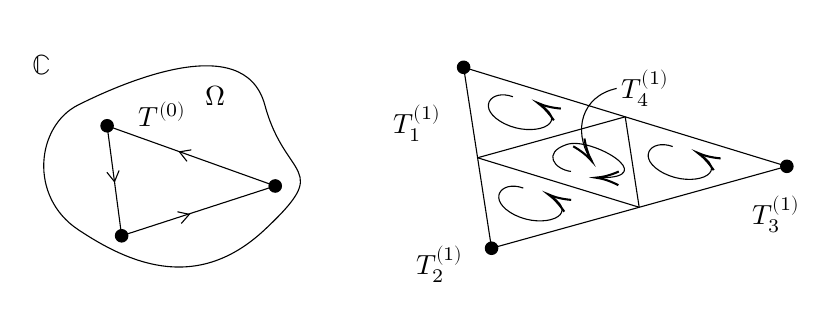
\begin{tikzpicture}[x=0.75pt,y=0.75pt,yscale=-1,xscale=1]
%uncomment if require: \path (0,300); %set diagram left start at 0, and has height of 300

%Shape: Polygon Curved [id:ds3386289484488558] 
\draw   (133,115) .. controls (153,105) and (213,78) .. (223,115) .. controls (233,152) and (256,144) .. (223,175) .. controls (190,206) and (157,191) .. (133,175) .. controls (109,159) and (113,125) .. (133,115) -- cycle ;
%Shape: Circle [id:dp40593013333768546] 
\draw  [fill={rgb, 255:red, 0; green, 0; blue, 0 }  ,fill opacity=1 ] (144,125) .. controls (144,123.34) and (145.34,122) .. (147,122) .. controls (148.66,122) and (150,123.34) .. (150,125) .. controls (150,126.66) and (148.66,128) .. (147,128) .. controls (145.34,128) and (144,126.66) .. (144,125) -- cycle ;
%Shape: Circle [id:dp8516576087175576] 
\draw  [fill={rgb, 255:red, 0; green, 0; blue, 0 }  ,fill opacity=1 ] (151,178) .. controls (151,176.34) and (152.34,175) .. (154,175) .. controls (155.66,175) and (157,176.34) .. (157,178) .. controls (157,179.66) and (155.66,181) .. (154,181) .. controls (152.34,181) and (151,179.66) .. (151,178) -- cycle ;
%Shape: Circle [id:dp1140813492392001] 
\draw  [fill={rgb, 255:red, 0; green, 0; blue, 0 }  ,fill opacity=1 ] (225,154) .. controls (225,152.34) and (226.34,151) .. (228,151) .. controls (229.66,151) and (231,152.34) .. (231,154) .. controls (231,155.66) and (229.66,157) .. (228,157) .. controls (226.34,157) and (225,155.66) .. (225,154) -- cycle ;
%Straight Lines [id:da32271189201063355] 
\draw    (147,125) -- (154,178) ;
%Straight Lines [id:da9881466923959998] 
\draw    (147,125) -- (228,154) ;
%Straight Lines [id:da33756092924141434] 
\draw    (154,178) -- (228,154) ;
\draw   (152.77,146.56) -- (150.57,151.93) -- (146.91,147.42) ;
\draw   (180.91,166.43) -- (186.58,167.68) -- (182.76,172.06) ;
\draw   (185.48,142.12) -- (181.87,137.57) -- (187.6,136.59) ;
%Straight Lines [id:da547604343128484] 
\draw    (318.77,96.83) -- (332.23,184) ;
%Straight Lines [id:da7089081413603506] 
\draw    (318.77,96.83) -- (474.5,144.53) ;
%Straight Lines [id:da6210680788690337] 
\draw    (332.23,184) -- (474.5,144.53) ;
%Shape: Circle [id:dp2445074927611688] 
\draw  [fill={rgb, 255:red, 0; green, 0; blue, 0 }  ,fill opacity=1 ] (329.23,184) .. controls (329.23,182.34) and (330.57,181) .. (332.23,181) .. controls (333.88,181) and (335.23,182.34) .. (335.23,184) .. controls (335.23,185.66) and (333.88,187) .. (332.23,187) .. controls (330.57,187) and (329.23,185.66) .. (329.23,184) -- cycle ;
%Shape: Circle [id:dp17785732571793123] 
\draw  [fill={rgb, 255:red, 0; green, 0; blue, 0 }  ,fill opacity=1 ] (315.77,96.83) .. controls (315.77,95.17) and (317.11,93.83) .. (318.77,93.83) .. controls (320.42,93.83) and (321.77,95.17) .. (321.77,96.83) .. controls (321.77,98.49) and (320.42,99.83) .. (318.77,99.83) .. controls (317.11,99.83) and (315.77,98.49) .. (315.77,96.83) -- cycle ;
%Shape: Circle [id:dp21699409783697265] 
\draw  [fill={rgb, 255:red, 0; green, 0; blue, 0 }  ,fill opacity=1 ] (471.5,144.53) .. controls (471.5,142.87) and (472.84,141.53) .. (474.5,141.53) .. controls (476.16,141.53) and (477.5,142.87) .. (477.5,144.53) .. controls (477.5,146.18) and (476.16,147.53) .. (474.5,147.53) .. controls (472.84,147.53) and (471.5,146.18) .. (471.5,144.53) -- cycle ;
%Straight Lines [id:da7735198491738475] 
\draw    (396.63,120.68) -- (325.5,140.41) ;
%Straight Lines [id:da5945755907993049] 
\draw    (325.5,140.41) -- (403.36,164.26) ;
%Straight Lines [id:da020720299680464294] 
\draw    (396.63,120.68) -- (403.36,164.26) ;
%Curve Lines [id:da5375121582011133] 
\draw    (392.5,107) .. controls (375.22,110.84) and (371.76,127.58) .. (379.48,140.42) ;
\draw [shift={(380.5,142)}, rotate = 235.3] [color={rgb, 255:red, 0; green, 0; blue, 0 }  ][line width=0.75]    (10.93,-3.29) .. controls (6.95,-1.4) and (3.31,-0.3) .. (0,0) .. controls (3.31,0.3) and (6.95,1.4) .. (10.93,3.29)   ;
%Curve Lines [id:da5821001759734961] 
\draw    (419.5,135) .. controls (408.5,131) and (401.5,141) .. (415.5,148) .. controls (429.01,154.76) and (447.18,148.47) .. (433.15,139.04) ;
\draw [shift={(431.5,138)}, rotate = 390.47] [color={rgb, 255:red, 0; green, 0; blue, 0 }  ][line width=0.75]    (10.93,-3.29) .. controls (6.95,-1.4) and (3.31,-0.3) .. (0,0) .. controls (3.31,0.3) and (6.95,1.4) .. (10.93,3.29)   ;
%Curve Lines [id:da8496780735582994] 
\draw    (370.5,147) .. controls (362.5,146) and (356.5,138) .. (368.5,134) .. controls (380.26,130.08) and (414.11,150.17) .. (384.4,150.03) ;
\draw [shift={(382.5,150)}, rotate = 361.74] [color={rgb, 255:red, 0; green, 0; blue, 0 }  ][line width=0.75]    (10.93,-3.29) .. controls (6.95,-1.4) and (3.31,-0.3) .. (0,0) .. controls (3.31,0.3) and (6.95,1.4) .. (10.93,3.29)   ;
%Curve Lines [id:da10315513416205713] 
\draw    (347.5,155) .. controls (336.5,151) and (329.5,161) .. (343.5,168) .. controls (357.01,174.76) and (375.18,168.47) .. (361.15,159.04) ;
\draw [shift={(359.5,158)}, rotate = 390.47] [color={rgb, 255:red, 0; green, 0; blue, 0 }  ][line width=0.75]    (10.93,-3.29) .. controls (6.95,-1.4) and (3.31,-0.3) .. (0,0) .. controls (3.31,0.3) and (6.95,1.4) .. (10.93,3.29)   ;
%Curve Lines [id:da00390300926240128] 
\draw    (342.5,111) .. controls (331.5,107) and (324.5,117) .. (338.5,124) .. controls (352.01,130.76) and (370.18,124.47) .. (356.15,115.04) ;
\draw [shift={(354.5,114)}, rotate = 390.47] [color={rgb, 255:red, 0; green, 0; blue, 0 }  ][line width=0.75]    (10.93,-3.29) .. controls (6.95,-1.4) and (3.31,-0.3) .. (0,0) .. controls (3.31,0.3) and (6.95,1.4) .. (10.93,3.29)   ;

% Text Node
\draw (193,104.4) node [anchor=north west][inner sep=0.75pt]    {$\Omega $};
% Text Node
\draw (110,89.4) node [anchor=north west][inner sep=0.75pt]    {$\mathbb{C}$};
% Text Node
\draw (161,112.4) node [anchor=north west][inner sep=0.75pt]    {$T^{( 0)}$};
% Text Node
\draw (283.6,113.65) node [anchor=north west][inner sep=0.75pt]    {$T^{( 1)}_{1}$};
% Text Node
\draw (294.6,181.65) node [anchor=north west][inner sep=0.75pt]    {$T^{( 1)}_{2}$};
% Text Node
\draw (456.6,157.65) node [anchor=north west][inner sep=0.75pt]    {$T^{( 1)}_{3}$};
% Text Node
\draw (393.6,96.65) node [anchor=north west][inner sep=0.75pt]    {$T^{( 1)}_{4}$};


\end{tikzpicture}
\end{center}

Then, \[\ointctrclockwise_{T^{(0)}} f(z) \dd z = 
  \ointctrclockwise_{T_1^{(1)}} f(z) \dd z + \ointctrclockwise_{T_2^{(1)}} f(z) \dd z
  + \ointctrclockwise_{T_3^{(1)}} f(z) \dd z + \ointctrclockwise_{T_4^{(1)}} f(z) \dd z.\]
By choosing \(j\) such that
\(\left|\ointctrclockwise_{T_j^{(1)}} f(z) \dd z\right|\) is the maximum
among the four integrals, we have
\[\left|\ointctrclockwise_{T^{(0)}} f(z) \dd z\right| 
  \le 4\left|\ointctrclockwise_{T_j^{(1)}} f(z) \dd z\right|.\] Now, by
renaming \(T_j^{(1)} = T^{(1)}\), we observe that
\[d^{(1)} = \frac{1}{2}d^{(0)}; \hspace{2mm} p^{(1)} = \frac{1}{2}p^{(0)}.\]
So, by repeating this process, we obtain a sequence of triangles
\(T^{(0)}, T^{(1)}, T^{(2)}, \cdots, T^{(n)}, \cdots\) such that
\[\left|\ointctrclockwise_{T^{(0)}} f(z) \dd z\right| 
  \le 4^n\left|\ointctrclockwise_{T^{(n)}} f(z) \dd z\right|,\] and
\[d^{(n)} = 2^{-n} d^{(0)}; \hspace{2mm} p^{(n)} = 2^{-n} p^{(0)},\]
where \(d^{(n)}, p^{(n)}\) denote the diameter and perimeter of
\(T^{(n)}\) respectively.

Now, by denoting \(\Omega^{(n)}\) be the closed region enclosed by
\(T^{n}\) so that \(\partial \Omega^{(n)} = T^{(n)}\), we have a
sequence of nested nonempty compact sets
\(\Omega^{(0)} \supseteq \Omega^{(1)} \supseteq \cdots\) whose diameter
tends to 0. So, due to results from metric spaces, there exists a unique
point \(z_0\) belonging to \(\bigcap \Omega^{(n)}\). Since \(f\) is
holomorphic, \[f(z) = f(z_0) + f'(z_0)(z - z_0) + (z - z_0) \psi(z)\]
where \(\psi\) is a function such that \(\psi(z) \to 0\) as
\(z \to z_0\).

Since \(f(z_0) + f'(z_0)(z - z_0)\) is simply a linear function, and
thus has a primitive, integrating it over a closed curve will result in
0, and so,
\[\ointctrclockwise_{T^{(n)}} f(z) \dd z = \ointctrclockwise_{T^{(n)}}\psi(z)(z - z_0) \dd z.\]
Now as \(z_0 \in \bigcap \Omega^{(n)}\), \(|z - z_0| \le d^{(n)}\), and
so, by ML-inequality,
\[\left| \ointctrclockwise_{T^{(n)}} f(z) \dd z \right| \le \epsilon_n d^{(n)}p^{(n)},\]
where \(\epsilon := \sup_{z \in T^{(n)}}|\psi(z)| \to 0\) as
\(n \to \infty\). Therefore
\[\left|\ointctrclockwise_{T^{(0)}} f(z) \dd z\right| 
  \le 4^n\left|\ointctrclockwise_{T^{(n)}} f(z) \dd z\right|
  \le \epsilon_n 4^n 2^{-n}d^{(0)} 2^{-n}p^{(0)} \to 0,\] as
\(n \to 0\). \qed

From this theorem, we see that all curves whose shapes are polygons also
satisfy Cauchy's theorem. That is, if \(\Omega \subseteq \mathbb{C}\) is
a open set, \(\gamma \subseteq \Omega\) is a curve describing a polygon,
and \(\Omega\) contains the interior of \(\gamma\), then, if \(f\) is
holomorphic on \(\Omega\), \[\oint_\gamma f(z) \dd z = 0.\] Indeed, this
is true since we can partition any polygon into smaller triangles such
that the values from the inner edges cancel, resulting in the total
integral to become zero. In fact, a stronger statement is true -- the
integral of a holomorphic function over any piecewise \(C^1\) curve on a
simply connected domain (which we will discuss in the next section)
vanishes.

\begin{theorem}[Local Existence of Primitives]
  A holomorphic function in an open disc has a primitive in that disc.
\end{theorem}
\proof

Wlog. let us assume that the disc \(D\) is centred at the origin. Then,
for all \(z \in D\), we consider the curve
\(\gamma_z :=  [0, \text{Re}(z)] \cup \{\text{Re}(z) + ti \mid t \in [0, \text{Im}(z)] \}\),
that is the right-angled curve connecting the origin with \(z\)
following the real axis. Now, as \(\gamma_z\) is piecewise continuous,
we may define \[F(z) := \int_{\gamma_z} f(w) \dd w.\] Consider the
difference,
\[F(z + h) - F(z) = \int_{\gamma_{z + h}} f(w) \dd w - \int_{\gamma_z} f(w) \dd w,\]
by the diagram below, we find that the difference is in fact the
integral along the straight line from \(z\) to \(z + h\).

\begin{center}
\tikzset{every picture/.style={line width=0.75pt}} %set default line width to 0.75pt        

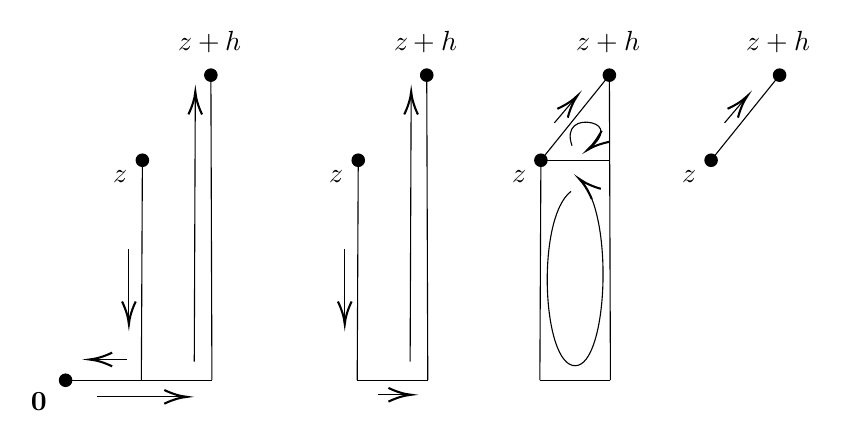
\begin{tikzpicture}[x=0.75pt,y=0.75pt,yscale=-1,xscale=1]
%uncomment if require: \path (0,300); %set diagram left start at 0, and has height of 300

%Shape: Circle [id:dp027258775303021787] 
\draw  [fill={rgb, 255:red, 0; green, 0; blue, 0 }  ,fill opacity=1 ] (197,94) .. controls (197,92.34) and (198.34,91) .. (200,91) .. controls (201.66,91) and (203,92.34) .. (203,94) .. controls (203,95.66) and (201.66,97) .. (200,97) .. controls (198.34,97) and (197,95.66) .. (197,94) -- cycle ;
%Shape: Circle [id:dp4860880282387001] 
\draw  [fill={rgb, 255:red, 0; green, 0; blue, 0 }  ,fill opacity=1 ] (164,135) .. controls (164,133.34) and (165.34,132) .. (167,132) .. controls (168.66,132) and (170,133.34) .. (170,135) .. controls (170,136.66) and (168.66,138) .. (167,138) .. controls (165.34,138) and (164,136.66) .. (164,135) -- cycle ;
%Shape: Circle [id:dp659691031475939] 
\draw  [fill={rgb, 255:red, 0; green, 0; blue, 0 }  ,fill opacity=1 ] (127,241) .. controls (127,239.34) and (128.34,238) .. (130,238) .. controls (131.66,238) and (133,239.34) .. (133,241) .. controls (133,242.66) and (131.66,244) .. (130,244) .. controls (128.34,244) and (127,242.66) .. (127,241) -- cycle ;
%Straight Lines [id:da9161997899342504] 
\draw    (130,241) -- (200.5,241) ;
%Straight Lines [id:da4628328210283985] 
\draw    (200,94) -- (200.5,241) ;
%Straight Lines [id:da24531528857425577] 
\draw    (167,135) -- (166.5,241) ;
%Straight Lines [id:da06293938710161817] 
\draw    (145,249) -- (186.5,249) ;
\draw [shift={(188.5,249)}, rotate = 180] [color={rgb, 255:red, 0; green, 0; blue, 0 }  ][line width=0.75]    (10.93,-3.29) .. controls (6.95,-1.4) and (3.31,-0.3) .. (0,0) .. controls (3.31,0.3) and (6.95,1.4) .. (10.93,3.29)   ;
%Straight Lines [id:da7020229409080956] 
\draw    (160.5,178) -- (160.5,212) ;
\draw [shift={(160.5,214)}, rotate = 270] [color={rgb, 255:red, 0; green, 0; blue, 0 }  ][line width=0.75]    (10.93,-3.29) .. controls (6.95,-1.4) and (3.31,-0.3) .. (0,0) .. controls (3.31,0.3) and (6.95,1.4) .. (10.93,3.29)   ;
%Straight Lines [id:da016203751378052855] 
\draw    (192,232) -- (192.49,104) ;
\draw [shift={(192.5,102)}, rotate = 450.22] [color={rgb, 255:red, 0; green, 0; blue, 0 }  ][line width=0.75]    (10.93,-3.29) .. controls (6.95,-1.4) and (3.31,-0.3) .. (0,0) .. controls (3.31,0.3) and (6.95,1.4) .. (10.93,3.29)   ;
%Straight Lines [id:da07762869882674939] 
\draw    (159.5,231) -- (143.5,231) ;
\draw [shift={(141.5,231)}, rotate = 360] [color={rgb, 255:red, 0; green, 0; blue, 0 }  ][line width=0.75]    (10.93,-3.29) .. controls (6.95,-1.4) and (3.31,-0.3) .. (0,0) .. controls (3.31,0.3) and (6.95,1.4) .. (10.93,3.29)   ;
%Shape: Circle [id:dp5305095359029792] 
\draw  [fill={rgb, 255:red, 0; green, 0; blue, 0 }  ,fill opacity=1 ] (301,94) .. controls (301,92.34) and (302.34,91) .. (304,91) .. controls (305.66,91) and (307,92.34) .. (307,94) .. controls (307,95.66) and (305.66,97) .. (304,97) .. controls (302.34,97) and (301,95.66) .. (301,94) -- cycle ;
%Shape: Circle [id:dp8680672367699809] 
\draw  [fill={rgb, 255:red, 0; green, 0; blue, 0 }  ,fill opacity=1 ] (268,135) .. controls (268,133.34) and (269.34,132) .. (271,132) .. controls (272.66,132) and (274,133.34) .. (274,135) .. controls (274,136.66) and (272.66,138) .. (271,138) .. controls (269.34,138) and (268,136.66) .. (268,135) -- cycle ;
%Straight Lines [id:da2520438705650401] 
\draw    (270.5,241) -- (304.5,241) ;
%Straight Lines [id:da9600987515534023] 
\draw    (304,94) -- (304.5,241) ;
%Straight Lines [id:da6867762927944552] 
\draw    (271,135) -- (270.5,241) ;
%Straight Lines [id:da4506690694374482] 
\draw    (280.5,248) -- (294.5,248) ;
\draw [shift={(296.5,248)}, rotate = 180] [color={rgb, 255:red, 0; green, 0; blue, 0 }  ][line width=0.75]    (10.93,-3.29) .. controls (6.95,-1.4) and (3.31,-0.3) .. (0,0) .. controls (3.31,0.3) and (6.95,1.4) .. (10.93,3.29)   ;
%Straight Lines [id:da3493360904429266] 
\draw    (264.5,178) -- (264.5,212) ;
\draw [shift={(264.5,214)}, rotate = 270] [color={rgb, 255:red, 0; green, 0; blue, 0 }  ][line width=0.75]    (10.93,-3.29) .. controls (6.95,-1.4) and (3.31,-0.3) .. (0,0) .. controls (3.31,0.3) and (6.95,1.4) .. (10.93,3.29)   ;
%Straight Lines [id:da6622622626510641] 
\draw    (296,232) -- (296.49,104) ;
\draw [shift={(296.5,102)}, rotate = 450.22] [color={rgb, 255:red, 0; green, 0; blue, 0 }  ][line width=0.75]    (10.93,-3.29) .. controls (6.95,-1.4) and (3.31,-0.3) .. (0,0) .. controls (3.31,0.3) and (6.95,1.4) .. (10.93,3.29)   ;
%Shape: Circle [id:dp8416922817175956] 
\draw  [fill={rgb, 255:red, 0; green, 0; blue, 0 }  ,fill opacity=1 ] (389,94) .. controls (389,92.34) and (390.34,91) .. (392,91) .. controls (393.66,91) and (395,92.34) .. (395,94) .. controls (395,95.66) and (393.66,97) .. (392,97) .. controls (390.34,97) and (389,95.66) .. (389,94) -- cycle ;
%Shape: Circle [id:dp37453124478890865] 
\draw  [fill={rgb, 255:red, 0; green, 0; blue, 0 }  ,fill opacity=1 ] (356,135) .. controls (356,133.34) and (357.34,132) .. (359,132) .. controls (360.66,132) and (362,133.34) .. (362,135) .. controls (362,136.66) and (360.66,138) .. (359,138) .. controls (357.34,138) and (356,136.66) .. (356,135) -- cycle ;
%Straight Lines [id:da8764037381694731] 
\draw    (358.5,241) -- (392.5,241) ;
%Straight Lines [id:da7292251610568219] 
\draw    (392,94) -- (392.5,241) ;
%Straight Lines [id:da16338914034450203] 
\draw    (359,135) -- (358.5,241) ;
%Straight Lines [id:da21913175509822036] 
\draw    (359,135) -- (392.5,135) ;
%Straight Lines [id:da6532179622634124] 
\draw    (359,135) -- (392,94) ;
%Curve Lines [id:da660412204704919] 
\draw    (373.5,150) .. controls (356.5,163) and (359.5,234) .. (375.5,234) .. controls (391.1,234) and (394.34,162.7) .. (378.74,145.24) ;
\draw [shift={(377.5,144)}, rotate = 401.41999999999996] [color={rgb, 255:red, 0; green, 0; blue, 0 }  ][line width=0.75]    (10.93,-3.29) .. controls (6.95,-1.4) and (3.31,-0.3) .. (0,0) .. controls (3.31,0.3) and (6.95,1.4) .. (10.93,3.29)   ;
%Curve Lines [id:da5400526552371321] 
\draw    (374,128) .. controls (370.66,118.75) and (377.11,115.48) .. (383.5,117) .. controls (389.48,118.42) and (389.52,123.3) .. (382.96,128.84) ;
\draw [shift={(381.5,130)}, rotate = 323.13] [color={rgb, 255:red, 0; green, 0; blue, 0 }  ][line width=0.75]    (10.93,-3.29) .. controls (6.95,-1.4) and (3.31,-0.3) .. (0,0) .. controls (3.31,0.3) and (6.95,1.4) .. (10.93,3.29)   ;
%Straight Lines [id:da35921857214953556] 
\draw    (365.5,117) -- (375.21,105.53) ;
\draw [shift={(376.5,104)}, rotate = 490.24] [color={rgb, 255:red, 0; green, 0; blue, 0 }  ][line width=0.75]    (10.93,-3.29) .. controls (6.95,-1.4) and (3.31,-0.3) .. (0,0) .. controls (3.31,0.3) and (6.95,1.4) .. (10.93,3.29)   ;
%Shape: Circle [id:dp21005530913264558] 
\draw  [fill={rgb, 255:red, 0; green, 0; blue, 0 }  ,fill opacity=1 ] (471,94) .. controls (471,92.34) and (472.34,91) .. (474,91) .. controls (475.66,91) and (477,92.34) .. (477,94) .. controls (477,95.66) and (475.66,97) .. (474,97) .. controls (472.34,97) and (471,95.66) .. (471,94) -- cycle ;
%Shape: Circle [id:dp6756758733196562] 
\draw  [fill={rgb, 255:red, 0; green, 0; blue, 0 }  ,fill opacity=1 ] (438,135) .. controls (438,133.34) and (439.34,132) .. (441,132) .. controls (442.66,132) and (444,133.34) .. (444,135) .. controls (444,136.66) and (442.66,138) .. (441,138) .. controls (439.34,138) and (438,136.66) .. (438,135) -- cycle ;
%Straight Lines [id:da17476796984102316] 
\draw    (441,135) -- (474,94) ;
%Straight Lines [id:da013336567431659896] 
\draw    (447.5,117) -- (457.21,105.53) ;
\draw [shift={(458.5,104)}, rotate = 490.24] [color={rgb, 255:red, 0; green, 0; blue, 0 }  ][line width=0.75]    (10.93,-3.29) .. controls (6.95,-1.4) and (3.31,-0.3) .. (0,0) .. controls (3.31,0.3) and (6.95,1.4) .. (10.93,3.29)   ;

% Text Node
\draw (112,245.4) node [anchor=north west][inner sep=0.75pt]    {$\mathbf{0}$};
% Text Node
\draw (152,138.4) node [anchor=north west][inner sep=0.75pt]    {$z$};
% Text Node
\draw (183,71.4) node [anchor=north west][inner sep=0.75pt]    {$z+h$};
% Text Node
\draw (256,138.4) node [anchor=north west][inner sep=0.75pt]    {$z$};
% Text Node
\draw (287,71.4) node [anchor=north west][inner sep=0.75pt]    {$z+h$};
% Text Node
\draw (344,138.4) node [anchor=north west][inner sep=0.75pt]    {$z$};
% Text Node
\draw (375,71.4) node [anchor=north west][inner sep=0.75pt]    {$z+h$};
% Text Node
\draw (426,138.4) node [anchor=north west][inner sep=0.75pt]    {$z$};
% Text Node
\draw (457,71.4) node [anchor=north west][inner sep=0.75pt]    {$z+h$};

\end{tikzpicture}
\end{center}

By denoting the straight line segment by \(\eta\), we have
\[F(z + h) - F(z) = \int_\eta f(w) \dd w.\] Now, as \(f\) is holomorphic
at \(z\), it is also continuous at \(z\), and so
\(f(w) = f(z) + \psi(w)\) for some function \(\psi\) where
\(\psi(w) \to 0\) as \(w \to z\). So,
\[F(z + h) - F(z) = \int_\eta f(z) \dd w + \int_\eta \psi(w) \dd w = 
  f(z) h + \int_\eta \psi(w) \dd w.\] Thus, by using the ML-inequality,
\[\left| \int_\eta \psi(w) \dd w \right| \le |h| \sup_{w \in \eta} |\psi(w)|,\]
where the right hand side tends to \(0\) as \(w \to z\). So,
\[\lim_{h \to 0} \frac{F(z + h) - F(z)}{h} = \lim_{h \to 0}\frac{f(z)h}{h} = f(z),\]
and hence, \(F\) is the primitive of \(f\). \qed

A direct corollary of this is the following.

\begin{corollary}[Cauchy-Goursat Theorem for a Disk]
  If \(f\) is holomorphic on a disc \(D\), then 
  \[\oint_\gamma f(z) \dd z = 0,\]
  for all closed curve \(\gamma \subseteq D\).
\end{corollary}

Similarly, the same can be said about a holomorphic function whose
domain contains a disc. That is, if \(f\) is holomorphic on the open set
\(\Omega\) which contains the circle \(C\) and its interior, then
\[\oint_C f(z) \dd z = 0.\] To see why this is true, we see that, as
\(\Omega\) is open, there exists a larger disk containing \(C\) which
\(f\) is holomorphic on, and so, the result follows.

\hypertarget{homotopies}{%
\subsection{Homotopies}\label{homotopies}}

\begin{definition}[Homotopic]
  Let \(\gamma_0, \gamma_1\) be curves in \(\Omega \subseteq \mathbb{C}\) with 
  common end-points, that is if \(\gamma_0\) and \(\gamma_1\) are two parametrisations 
  defined on \([a, b]\), then \(\gamma_0(a) = \gamma_1(a) = \alpha\) and 
  \(\gamma_0(b) = \gamma_0(b) = \beta\). Then, we say \(\gamma_0\) and \(\gamma_1\) are 
  homotopic in \(\Omega\), if for all \(s \in [0, 1]\) there exists some curve 
  \(\gamma_s \subseteq \Omega\) with parametrisation \(\gamma_s : [a, b] \to \Omega\) 
  such that 
  \[\gamma_s(a) = \alpha; \hspace{2mm} \gamma_s(b) = \beta,\]
  and for all \(t \in [a, b]\), 
  \[\gamma_s(t) \mid_{s = 0} = \gamma_0(t); \hspace{2mm} \gamma_s(t) \mid_{s = 1} = \gamma_1(t).\]
  Moreover, \(\gamma_s(t)\) is jointly continuous with respect to \(s\) and \(t\).
\end{definition}

Homotopic curves forms an equivalence relations on the set of curves and
processes some very ``nice'' properties.

\begin{prop}
  If \(\gamma_0\) and \(\gamma_1\) are two homotopic curves, and 
  \(f : \Omega \to \mathbb{C}\) is holomorphic on the open set \(\Omega\), then 
  \[\int_{\gamma_0} f(z) \dd z = \int_{\gamma_1} f(z) \dd z.\]
\end{prop}
\proof

If \(\gamma_s(t)\) is the homotopy between \(\gamma_0\) and
\(\gamma_1\), then we can define the continuous function
\[F(s, t) : [0, 1] \times [a, b] \to \Omega : (s, t) \mapsto \gamma_s(t).\]
Since \(F\) is continuous, and by Heine-Borel \([0, 1] \times [a, b]\)
is compact, the image of \(F\) is also compact and we shall denote it by
\(\mathcal{K} \subseteq \Omega\).

Now, since \(\Omega\) is open, for all \(p \in \mathcal{K}\), there
exists some \(\epsilon_p > 0\) such that
\(D_{\epsilon_p}(p) \subseteq \Omega\). Thus, we may construct the open
cover \(\mathcal{C} := \{D_{\epsilon_p}(p) \mid p \in \mathcal{K}\}\),
and so, by compactness, we may find a finite subcover of \(\mathcal{C}\)
allowing us to choose \(\epsilon > 0\) such that for all
\(p \in \mathcal{K}\), \(D_{3\epsilon}(p) \subseteq \Omega\).

Furthermore, as \(F\) is uniformly continuous, there exists some
\(\delta\), such that for all \(s_1, s_2 \in \Omega\),
\(|s_1 - s_2| < \delta\), then
\[\sup_{t \in [a, b]} |\gamma_{s_1}(t) - \gamma_{s_2}(t)| < \epsilon.\]
So, we may choose discs \(\{D_0, \cdots, D_n\}\) of radius \(2\epsilon\)
and points \(\{z_0, \cdots, z_{n + 1}\} \subseteq \gamma_{s_1}\) and
\(\{w_0, \cdots, w_{n + 1}\} \subseteq \gamma_{s_2}\) such that
\(\gamma_{s_1} \cup \gamma_{s_2} \subseteq \bigcup D_i\) and
\[z_i, z_{i + 1}, w_i, w_{i + 1} \in D_i.\]

\begin{center}
  
\tikzset{every picture/.style={line width=0.75pt}} %set default line width to 0.75pt        

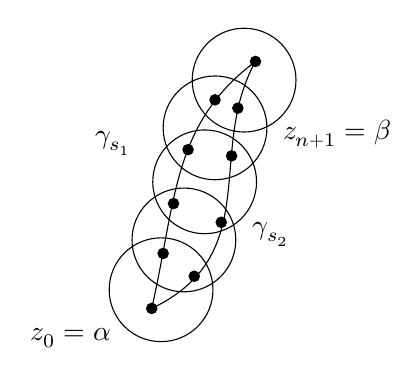
\begin{tikzpicture}[x=0.75pt,y=0.75pt,yscale=-1,xscale=1]
%uncomment if require: \path (0,300); %set diagram left start at 0, and has height of 300

%Curve Lines [id:da8047429829011434] 
\draw    (235.5,193) .. controls (290,167) and (261.5,117) .. (285.5,74) ;
%Curve Lines [id:da3790761664602649] 
\draw    (235.5,193) .. controls (247.5,140) and (245.5,104) .. (285.5,74) ;
%Shape: Circle [id:dp7582243054036091] 
\draw   (215,184) .. controls (215,170.19) and (226.19,159) .. (240,159) .. controls (253.81,159) and (265,170.19) .. (265,184) .. controls (265,197.81) and (253.81,209) .. (240,209) .. controls (226.19,209) and (215,197.81) .. (215,184) -- cycle ;
%Shape: Circle [id:dp07975248214180919] 
\draw   (226,160) .. controls (226,146.19) and (237.19,135) .. (251,135) .. controls (264.81,135) and (276,146.19) .. (276,160) .. controls (276,173.81) and (264.81,185) .. (251,185) .. controls (237.19,185) and (226,173.81) .. (226,160) -- cycle ;
%Shape: Circle [id:dp3504063032449949] 
\draw   (236,132) .. controls (236,118.19) and (247.19,107) .. (261,107) .. controls (274.81,107) and (286,118.19) .. (286,132) .. controls (286,145.81) and (274.81,157) .. (261,157) .. controls (247.19,157) and (236,145.81) .. (236,132) -- cycle ;
%Shape: Circle [id:dp6901897328600055] 
\draw   (241,106) .. controls (241,92.19) and (252.19,81) .. (266,81) .. controls (279.81,81) and (291,92.19) .. (291,106) .. controls (291,119.81) and (279.81,131) .. (266,131) .. controls (252.19,131) and (241,119.81) .. (241,106) -- cycle ;
%Shape: Circle [id:dp1676188138277661] 
\draw  [fill={rgb, 255:red, 0; green, 0; blue, 0 }  ,fill opacity=1 ] (233,193) .. controls (233,191.62) and (234.12,190.5) .. (235.5,190.5) .. controls (236.88,190.5) and (238,191.62) .. (238,193) .. controls (238,194.38) and (236.88,195.5) .. (235.5,195.5) .. controls (234.12,195.5) and (233,194.38) .. (233,193) -- cycle ;
%Shape: Circle [id:dp347239256875163] 
\draw  [fill={rgb, 255:red, 0; green, 0; blue, 0 }  ,fill opacity=1 ] (238.5,166.5) .. controls (238.5,165.12) and (239.62,164) .. (241,164) .. controls (242.38,164) and (243.5,165.12) .. (243.5,166.5) .. controls (243.5,167.88) and (242.38,169) .. (241,169) .. controls (239.62,169) and (238.5,167.88) .. (238.5,166.5) -- cycle ;
%Shape: Circle [id:dp945891608957599] 
\draw   (255,83) .. controls (255,69.19) and (266.19,58) .. (280,58) .. controls (293.81,58) and (305,69.19) .. (305,83) .. controls (305,96.81) and (293.81,108) .. (280,108) .. controls (266.19,108) and (255,96.81) .. (255,83) -- cycle ;
%Shape: Circle [id:dp6219629034666561] 
\draw  [fill={rgb, 255:red, 0; green, 0; blue, 0 }  ,fill opacity=1 ] (253.5,177.5) .. controls (253.5,176.12) and (254.62,175) .. (256,175) .. controls (257.38,175) and (258.5,176.12) .. (258.5,177.5) .. controls (258.5,178.88) and (257.38,180) .. (256,180) .. controls (254.62,180) and (253.5,178.88) .. (253.5,177.5) -- cycle ;
%Shape: Circle [id:dp6907929228820959] 
\draw  [fill={rgb, 255:red, 0; green, 0; blue, 0 }  ,fill opacity=1 ] (266.5,151.5) .. controls (266.5,150.12) and (267.62,149) .. (269,149) .. controls (270.38,149) and (271.5,150.12) .. (271.5,151.5) .. controls (271.5,152.88) and (270.38,154) .. (269,154) .. controls (267.62,154) and (266.5,152.88) .. (266.5,151.5) -- cycle ;
%Shape: Circle [id:dp29296285573610015] 
\draw  [fill={rgb, 255:red, 0; green, 0; blue, 0 }  ,fill opacity=1 ] (243.5,142.5) .. controls (243.5,141.12) and (244.62,140) .. (246,140) .. controls (247.38,140) and (248.5,141.12) .. (248.5,142.5) .. controls (248.5,143.88) and (247.38,145) .. (246,145) .. controls (244.62,145) and (243.5,143.88) .. (243.5,142.5) -- cycle ;
%Shape: Circle [id:dp7152580667384663] 
\draw  [fill={rgb, 255:red, 0; green, 0; blue, 0 }  ,fill opacity=1 ] (250.5,116.5) .. controls (250.5,115.12) and (251.62,114) .. (253,114) .. controls (254.38,114) and (255.5,115.12) .. (255.5,116.5) .. controls (255.5,117.88) and (254.38,119) .. (253,119) .. controls (251.62,119) and (250.5,117.88) .. (250.5,116.5) -- cycle ;
%Shape: Circle [id:dp8822342438230766] 
\draw  [fill={rgb, 255:red, 0; green, 0; blue, 0 }  ,fill opacity=1 ] (271.5,119.5) .. controls (271.5,118.12) and (272.62,117) .. (274,117) .. controls (275.38,117) and (276.5,118.12) .. (276.5,119.5) .. controls (276.5,120.88) and (275.38,122) .. (274,122) .. controls (272.62,122) and (271.5,120.88) .. (271.5,119.5) -- cycle ;
%Shape: Circle [id:dp06160409361528063] 
\draw  [fill={rgb, 255:red, 0; green, 0; blue, 0 }  ,fill opacity=1 ] (263.5,92.5) .. controls (263.5,91.12) and (264.62,90) .. (266,90) .. controls (267.38,90) and (268.5,91.12) .. (268.5,92.5) .. controls (268.5,93.88) and (267.38,95) .. (266,95) .. controls (264.62,95) and (263.5,93.88) .. (263.5,92.5) -- cycle ;
%Shape: Circle [id:dp2542021967684036] 
\draw  [fill={rgb, 255:red, 0; green, 0; blue, 0 }  ,fill opacity=1 ] (274.5,96.5) .. controls (274.5,95.12) and (275.62,94) .. (277,94) .. controls (278.38,94) and (279.5,95.12) .. (279.5,96.5) .. controls (279.5,97.88) and (278.38,99) .. (277,99) .. controls (275.62,99) and (274.5,97.88) .. (274.5,96.5) -- cycle ;
%Shape: Circle [id:dp09005339368588361] 
\draw  [fill={rgb, 255:red, 0; green, 0; blue, 0 }  ,fill opacity=1 ] (283,74) .. controls (283,72.62) and (284.12,71.5) .. (285.5,71.5) .. controls (286.88,71.5) and (288,72.62) .. (288,74) .. controls (288,75.38) and (286.88,76.5) .. (285.5,76.5) .. controls (284.12,76.5) and (283,75.38) .. (283,74) -- cycle ;

% Text Node
\draw (207,106.4) node [anchor=north west][inner sep=0.75pt]    {$\gamma _{s_{1}}$};
% Text Node
\draw (283,150.4) node [anchor=north west][inner sep=0.75pt]    {$\gamma _{s_{2}}$};
% Text Node
\draw (176,201.4) node [anchor=north west][inner sep=0.75pt]    {$z_{0} =\alpha $};
% Text Node
\draw (297.5,100.9) node [anchor=north west][inner sep=0.75pt]    {$z_{n + 1} =\beta $};

\end{tikzpicture}

\end{center}

Now, by the local existence of primitives, for each disc \(D_i\), there
exists some \(F_i\) such that \(F_i\) is the primitive of \(f\) on
\(D_i\). By observing that on \(D_i \cap D_{i + 1}\), \(F_i\) and
\(F_{i + 1}\) are both primitives to \(f\), they can only differ by a
constant (on \(D_i \cap D_{i + 1}\)). So,
\[F_{i + 1}(z_{i + 1}) - F_i(z_{i + 1}) = F_{i + 1}(w_{i + 1}) - F_i(w_{i + 1}),\]
and hence, \[\begin{split}
    \int_{\gamma_{s_1}}f(z) \dd z - \int_{\gamma_{s_2}} f(z) \dd z & = 
      \sum_{i = 0}^{n}(F_i(z_{i + 1}) - F_i(z_i)) - \sum_{i = 0}^n(F_i(w_{i + 1}) - F_i(w_i))\\
      & = \sum_{i = 0}^n(F_i(z_{i + 1}) - F_i(w_{i + 1}) - (F_i(z_i) - F_i(w_i)))\\
      & = F_n(z_{n + 1}) - F_n(w_{n + 1}) - (F_0(z_0) - F_0(w_0))\\
      & = F_n(\beta) - F_n(\beta) - (F_0(\alpha) - F_0(\alpha)) = 0
  \end{split}\] Finally, by dividing the interval \([0, 1]\) into
subintervals with size less than \(\delta\), we see that
\[\int_{\gamma_0} f(z) \dd z = \int_{\gamma_1} f(z) \dd z.\] \qed

\begin{definition}[Simply Connected]
  An open set \(\Omega \subseteq \mathbb{C}\) is simply connected if any two pairs 
  of curves with the same end points in \(\Omega\) are homotopic.
\end{definition}

Straight away, we see that a disc is connected as given two curves in a
disc \(\gamma_1, \gamma_2\), we have to homotopy
\(\gamma_s(t) = (1- s)\gamma_0(t) + s\gamma_1(t)\). Furthermore, by the
same argument we have any convex sets are also simply connected. On the
other hand, we see that any sets which contains a hole is not simply
connected.

As mentioned previously, the integral of a holomorphic function over any
closed curve on a simply connected set vanishes. This follows straight
way from the following theorem.

\begin{theorem}
  Any holomorphic function in a simply connected domain has a primitive.
\end{theorem}
\proof

Suppose \(f : \Omega \to \mathbb{C}\) is holomorphic with the simply
connected domain \(\Omega\). Then, let us fix a point \(z_0 \in \Omega\)
and define \[F(z) = \int_\gamma f(w) \dd w,\] where \(\gamma\) is any
curve in \(\Omega\) joining \(z_0\) to \(z\). We note that this
definition is independent of the specific choice of \(\gamma\) since
\(\Omega\) is simply connected. Consider,
\[F(z + h) - F(z) = \int_\eta f(w) \dd w,\] where \(\eta\) is the
straight line joining \(z\) and \(z + h\). By the same argument as our
proof for local existence of primitives, we find
\[\lim_{h \to 0} \frac{F(z + h) - F(h)}{h} = f(z),\] implying \(F\) is
the primitive of \(f\). \qed

\begin{corollary}[Cauchy-Goursat Theorem]
  Let \(\Omega\) be a simply connected domain and \(f : \Omega \to \mathbb{C}\) 
  be holomorphic on \(\Omega\). Then, if \(\gamma\) is a closed, piecewise-smooth 
  curve in \(\Omega\), 
  \[\oint_\gamma f(z) \dd z = 0.\]
\end{corollary}
\proof

Indeed, without using the existence of primitives, we see that we may
partition \(\gamma\) into two curves with the same end points, and so,
as \(\Omega\) is simply connected, they are also homotopic. Thus, the
integral over these two curves result in the same value. Now, by
reversing the orientation of one of these curves, we obtain our result.
\qed

\begin{theorem}[Deformation Theorem]
  Let \(\gamma_1, \gamma_2 \subseteq \Omega\) be two simple, closed, 
  piecewise-smooth curves with \(\gamma_2\) lying wholly inside \(\gamma_1\). 
  If \(f : \Omega \to \mathbb{C}\) is holomorphic in the domain containing the 
  region between \(\gamma_1\) and \(\gamma_2\), then 
  \[\ointctrclockwise_{\gamma_1} f(z) \dd z = \ointctrclockwise_{\gamma_2} f(z) \dd z.\]
\end{theorem}

\proof

We note that we cannot directly apply the Cauchy-Goursat theorem as
\(f\) is not necessarily holomorphic in the region enclosed by
\(\gamma_2\). Instead, we construct a bridge between \(\gamma_1\) and
\(\gamma_2\).

\begin{center}
  
\tikzset{every picture/.style={line width=0.75pt}} %set default line width to 0.75pt        

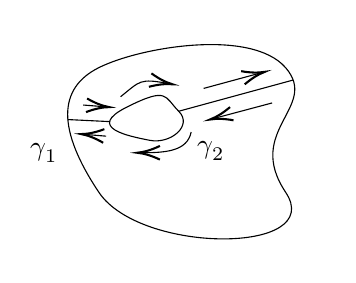
\begin{tikzpicture}[x=0.75pt,y=0.75pt,yscale=-1,xscale=1]
%uncomment if require: \path (0,300); %set diagram left start at 0, and has height of 300

%Shape: Polygon Curved [id:ds4133997265054681] 
\draw   (121,114) .. controls (141,104) and (194.5,95) .. (211,114) .. controls (227.5,133) and (191,144) .. (211,174) .. controls (231,204) and (141,204) .. (121,174) .. controls (101,144) and (101,124) .. (121,114) -- cycle ;
%Shape: Polygon Curved [id:ds7005624339900847] 
\draw   (134.5,133) .. controls (154.5,123) and (152.5,128) .. (159.5,135) .. controls (166.5,142) and (155.5,151) .. (145.5,149) .. controls (135.5,147) and (114.5,143) .. (134.5,133) -- cycle ;
%Straight Lines [id:da5284031136917495] 
\draw    (106,139) -- (126.5,140) ;
%Straight Lines [id:da7840043899366151] 
\draw    (159.5,135) -- (214.5,120) ;
%Straight Lines [id:da11905633800020321] 
\draw    (204.5,131) -- (176.43,138.48) ;
\draw [shift={(174.5,139)}, rotate = 345.07] [color={rgb, 255:red, 0; green, 0; blue, 0 }  ][line width=0.75]    (10.93,-3.29) .. controls (6.95,-1.4) and (3.31,-0.3) .. (0,0) .. controls (3.31,0.3) and (6.95,1.4) .. (10.93,3.29)   ;
%Curve Lines [id:da7328876171745344] 
\draw    (165.5,145) .. controls (163.61,154.45) and (152.79,154.97) .. (141.48,155) ;
\draw [shift={(139.5,155)}, rotate = 360] [color={rgb, 255:red, 0; green, 0; blue, 0 }  ][line width=0.75]    (10.93,-3.29) .. controls (6.95,-1.4) and (3.31,-0.3) .. (0,0) .. controls (3.31,0.3) and (6.95,1.4) .. (10.93,3.29)   ;
%Straight Lines [id:da2966290564718628] 
\draw    (124.5,147) -- (114.49,146.17) ;
\draw [shift={(112.5,146)}, rotate = 364.76] [color={rgb, 255:red, 0; green, 0; blue, 0 }  ][line width=0.75]    (10.93,-3.29) .. controls (6.95,-1.4) and (3.31,-0.3) .. (0,0) .. controls (3.31,0.3) and (6.95,1.4) .. (10.93,3.29)   ;
%Straight Lines [id:da3595647541786302] 
\draw    (113.5,132) -- (124.01,132.84) ;
\draw [shift={(126,133)}, rotate = 184.57] [color={rgb, 255:red, 0; green, 0; blue, 0 }  ][line width=0.75]    (10.93,-3.29) .. controls (6.95,-1.4) and (3.31,-0.3) .. (0,0) .. controls (3.31,0.3) and (6.95,1.4) .. (10.93,3.29)   ;
%Curve Lines [id:da31305351619211286] 
\draw    (131.5,128) .. controls (141.1,120.32) and (140.56,119.09) .. (154.66,121.66) ;
\draw [shift={(156.5,122)}, rotate = 190.62] [color={rgb, 255:red, 0; green, 0; blue, 0 }  ][line width=0.75]    (10.93,-3.29) .. controls (6.95,-1.4) and (3.31,-0.3) .. (0,0) .. controls (3.31,0.3) and (6.95,1.4) .. (10.93,3.29)   ;
%Straight Lines [id:da0871922023706333] 
\draw    (171.5,124) -- (199.07,116.52) ;
\draw [shift={(201,116)}, rotate = 524.8299999999999] [color={rgb, 255:red, 0; green, 0; blue, 0 }  ][line width=0.75]    (10.93,-3.29) .. controls (6.95,-1.4) and (3.31,-0.3) .. (0,0) .. controls (3.31,0.3) and (6.95,1.4) .. (10.93,3.29)   ;

% Text Node
\draw (87,149.4) node [anchor=north west][inner sep=0.75pt]    {$\gamma _{1}$};
% Text Node
\draw (167.5,148.4) node [anchor=north west][inner sep=0.75pt]    {$\gamma _{2}$};


\end{tikzpicture}

\end{center}

By considering the slices, we see that the sum of the integrals of \(f\)
over the top and bottom closed curves is simply
\[\ointctrclockwise_{\gamma_1} f(z) \dd z - \ointctrclockwise_{\gamma_2} f(z) \dd z.\]
However, as the region covered by the two curves are the same region
between \(\gamma_1\) and \(\gamma_2\), \(f\) is holomorphic on the
region enclosed by the two curves, and so, the integrals evaluates to
zero by Cauchy-Goursat's theorem and hence,
\[\ointctrclockwise_{\gamma_1} f(z) \dd z - \ointctrclockwise_{\gamma_2} f(z) \dd z = 0.\]
\qed

The deformation theorem is very useful whenever we are able to restrict
a difficult curve onto a simpler curve (such as a circle) and thus, have
a easier time to parametrise the integral. As an example consider the
following integral over the curve
\(\gamma = \{z \in \mathbb{C} \mid |z - 1| = 2\}\).
\[\oint_\gamma \frac{\dd z}{z^2 - 4} = \oint_\gamma \frac{\dd z}{(z - 2)(z + 2)} 
  = \frac{1}{4}\oint_\gamma \frac{1}{z - 2} - \frac{1}{z + 2} \dd z.\]
Since \(\frac{1}{z + 2}\) is holom orphic except at \(-2\) which is
outside of \(\gamma\), we have \[\oint_\gamma \frac{\dd z}{z + 2} = 0.\]
On the other hand, to evaluate \(\frac{1}{z - 2}\), by the deformation
theorem, we have
\[\oint_\gamma \frac{\dd z}{z - 2} = \oint_{\{z \mid |z - 2| = 1\}} \frac{\dd z}{z - 2} 
  = \oint_{C_1(0)} \frac{\dd w}{w} = 2\pi i.\] Thus,
\[\oint_\gamma \frac{\dd z}{z^2 - 4} = i \frac{\pi}{2}.\]

As another example, consider that we would like to show for all
\(\xi \in \mathbb{R}\),
\[e^{-\pi \xi^2} = \int_{-\infty}^\infty e^{-\pi x^2}e^{-2\pi i x \xi^2} \dd x.\]

Suppose \(\xi > 0\) (the argument for \(\xi <0\) is similar) and let
\(\gamma_R\) be the following curve as described in the diagram below
for some \(R \in \mathbb{R}^+\). As \(f(z) = e^{-\pi z^2}\) is entire,
by the Cauchy-Goursat theorem, we have
\[\oint_{\gamma_R} f(z) \dd z = 0.\]

\begin{center}

\tikzset{every picture/.style={line width=0.75pt}} %set default line width to 0.75pt        

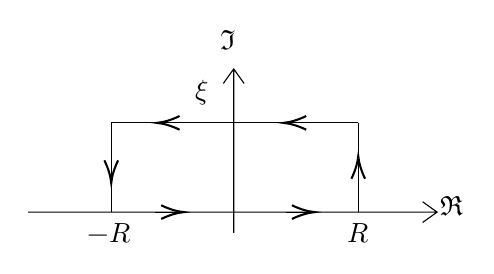
\begin{tikzpicture}[x=0.75pt,y=0.75pt,yscale=-1,xscale=1]
%uncomment if require: \path (0,300); %set diagram left start at 0, and has height of 300

%Shape: Axis 2D [id:dp07563419905194713] 
\draw  (111.5,133) -- (308.5,133)(210.5,64) -- (210.5,143) (301.5,128) -- (308.5,133) -- (301.5,138) (205.5,71) -- (210.5,64) -- (215.5,71)  ;
%Straight Lines [id:da7174628546578379] 
\draw    (270.5,90) -- (270.5,133) ;
%Straight Lines [id:da5322584315739751] 
\draw    (270.5,90) -- (151.5,90) ;
%Straight Lines [id:da6768293830789123] 
\draw    (151.5,90) -- (151.5,133) ;
%Straight Lines [id:da9919844180463244] 
\draw    (235.5,133) -- (247.5,133) ;
\draw [shift={(249.5,133)}, rotate = 180] [color={rgb, 255:red, 0; green, 0; blue, 0 }  ][line width=0.75]    (10.93,-3.29) .. controls (6.95,-1.4) and (3.31,-0.3) .. (0,0) .. controls (3.31,0.3) and (6.95,1.4) .. (10.93,3.29)   ;
%Straight Lines [id:da8963917719506822] 
\draw    (172.5,133) -- (184.5,133) ;
\draw [shift={(186.5,133)}, rotate = 180] [color={rgb, 255:red, 0; green, 0; blue, 0 }  ][line width=0.75]    (10.93,-3.29) .. controls (6.95,-1.4) and (3.31,-0.3) .. (0,0) .. controls (3.31,0.3) and (6.95,1.4) .. (10.93,3.29)   ;
%Straight Lines [id:da2552279489294458] 
\draw    (270.5,119) -- (270.5,108) ;
\draw [shift={(270.5,106)}, rotate = 450] [color={rgb, 255:red, 0; green, 0; blue, 0 }  ][line width=0.75]    (10.93,-3.29) .. controls (6.95,-1.4) and (3.31,-0.3) .. (0,0) .. controls (3.31,0.3) and (6.95,1.4) .. (10.93,3.29)   ;
%Straight Lines [id:da5361951267994474] 
\draw    (151.5,104) -- (151.5,117) ;
\draw [shift={(151.5,119)}, rotate = 270] [color={rgb, 255:red, 0; green, 0; blue, 0 }  ][line width=0.75]    (10.93,-3.29) .. controls (6.95,-1.4) and (3.31,-0.3) .. (0,0) .. controls (3.31,0.3) and (6.95,1.4) .. (10.93,3.29)   ;
%Straight Lines [id:da4731194124837399] 
\draw    (250.5,90) -- (236.5,90) ;
\draw [shift={(234.5,90)}, rotate = 360] [color={rgb, 255:red, 0; green, 0; blue, 0 }  ][line width=0.75]    (10.93,-3.29) .. controls (6.95,-1.4) and (3.31,-0.3) .. (0,0) .. controls (3.31,0.3) and (6.95,1.4) .. (10.93,3.29)   ;
%Straight Lines [id:da5725652743270169] 
\draw    (189.5,90) -- (175.5,90) ;
\draw [shift={(173.5,90)}, rotate = 360] [color={rgb, 255:red, 0; green, 0; blue, 0 }  ][line width=0.75]    (10.93,-3.29) .. controls (6.95,-1.4) and (3.31,-0.3) .. (0,0) .. controls (3.31,0.3) and (6.95,1.4) .. (10.93,3.29)   ;

% Text Node
\draw (139,137.4) node [anchor=north west][inner sep=0.75pt]    {$-R$};
% Text Node
\draw (264,137.4) node [anchor=north west][inner sep=0.75pt]    {$R$};
% Text Node
\draw (191,68.4) node [anchor=north west][inner sep=0.75pt]    {$\xi $};
% Text Node
\draw (309,124.4) node [anchor=north west][inner sep=0.75pt]    {$\Re $};
% Text Node
\draw (203,44.4) node [anchor=north west][inner sep=0.75pt]    {$\Im $};

\end{tikzpicture}

\end{center}

On the other hand, we have
\[\oint_{\gamma_R} f(z) \dd z = \int_{-R}^R f(x) \dd x + 
  \int_0^\xi f(R + iy) \dd y + \int_R^{-R} f(x + i\xi) \dd x
  + \int_\xi^0 f(-R + iy) \dd y.\] Consider \[\begin{split}
  \left| \int_0^\xi f(R + iy) \dd y \right| 
    & = \left|\int_0^\xi e^{-\pi(R + iy)^2} \dd y\right|
      = \left|\int_0^\xi e^{-\pi (R^2 - y^2 + 2iRy)} \dd y\right|\\
    & = |e^{-\pi R^2}| \left|\int_0^\xi e^{\pi y^2}e^{- 2i\pi Ry} \dd y\right|
      \le e^{-\pi R^2} \int_0^\xi |e^{\pi y^2}e^{- 2i\pi Ry}| \dd y\\
    & = e^{-\pi R^2} \int_0^\xi |e^{\pi y^2}| \dd y 
      \le  e^{-\pi R^2} \xi e^{\pi \xi^2}
\end{split}\] where the last inequality is due to the ML-indequality.
So, the integral tends to 0 as \(R \to \infty\). Similarly,
\(\left| \int_\xi^0 f(R + iy) \dd y \right| \to 0\) and so since
\(\lim_{R \to \infty} \int_{-R}^R f(x) \dd x = 1\) (the standard
Gaussian integral), \[\begin{split}
  0 & = \lim_{R \to \infty} \oint_{\gamma_R} f(z) \dd z 
      = 1 + \lim_{R \to \infty}\int_R^{-R} f(x + i\xi) \dd x 
      = 1 - \lim_{R \to \infty}\int_{-R}^{R} f(x + i\xi) \dd x \\
    & = 1 - \int_{-\infty}^\infty e^{-\pi(x + i\xi)^2}\dd x 
      = 1 - \int_{-\infty}^\infty e^{-\pi(x^2 + 2ix\xi - \xi^2)}\dd x
      = 1 - e^{\pi \xi^2}\int_{-\infty}^\infty e^{-\pi x^2} e^{-2\pi i x\xi}\dd x.
\end{split}\] So,
\[e^{-\pi \xi^2} = \int_{-\infty}^\infty e^{-\pi x^2} e^{-2\pi i x\xi}\dd x,\]
as required.

\newpage

\hypertarget{cauchys-integral-formula}{%
\section{Cauchy's Integral Formula}\label{cauchys-integral-formula}}

Cauchy's integral formulae is an amazing theorem that relates the value
of a holomorphic function with a special formula. Indeed, with the
Cauchy's integral formula, it is possible to find the value of \(f\) as
some point \(z_0\) just from the value of \(f\) on some neighbourhood.
We shall in this chapter investigate Cauchy's integral formula and some
of its applications.

\begin{theorem}[Cauchy's Integral Formula]
  Let \(f\) be holomorphic inside and on a simple, closed, piecewise-smooth 
  curve \(\gamma\). Then for any \(z_0\) interior to \(\gamma\), we have 
  \[f(z_0) = \frac{1}{2\pi i} \ointctrclockwise_\gamma \frac{f(z)}{z - z_0} \dd z.\]
\end{theorem}
\proof

As \(z_0 \in \gamma^\circ\) where \(\gamma^\circ\) is open, there exists
some \(r' > 0\) such that \(B_{r'}(z_0) \subseteq \gamma^\circ\).
Furthermroe, as \(f\) is holomorphic as \(z_0\), we have \(f\) is
continuous as \(z_0\). So by fixing \(\epsilon > 0\), there exists some
\(\delta > 0\), such that the continuity criterion applies. So, by
letting \(r :< \min\{r', \delta\}\), \(C := C_r(z_0)\) is a closed curve
fully inside of \(\gamma\) such that for all \(z \in D_r(z_0)\),
\[| f(z) - f(z_0) | < \epsilon.\] So, by the deformation theorem, we
have
\[\oint_\gamma \frac{f(z)}{z - z_0} \dd z = \oint_C \frac{f(z)}{z - z_0} \dd z.\]
Then, \[\begin{split}
    \frac{1}{2\pi i}\oint_C \frac{f(z)}{z - z_0} \dd z 
      & = \frac{f(z_0)}{2\pi i}\oint_C \frac{1}{z - z_0} \dd z 
        + \frac{1}{2\pi i}\oint_C \frac{f(z) - f(z_0)}{z - z_0} \dd z \\
      & = f(z_0) + \frac{1}{2\pi i}\oint_C \frac{f(z) - f(z_0)}{z - z_0} \dd z.
  \end{split}\] Now, consider, by the ML-inequality,
\[\left| \frac{1}{2\pi i}\oint_C \frac{f(z) - f(z_0)}{z - z_0} \dd z\right|
    \le \frac{1}{2\pi} \oint_C \left| \frac{f(z) - f(z_0)}{z - z_0} \right| \dd z
    \le \frac{1}{2\pi} \oint_C \frac{\epsilon}{r} \dd z
    = \frac{1}{2\pi} \frac{\epsilon}{r} 2\pi r = \epsilon.\] Since
\(\epsilon\) was arbitrary,
\[\frac{1}{2\pi i}\oint_C \frac{f(z) - f(z_0)}{z - z_0} \dd z = 0\] and
hence the result. \qed

\begin{theorem}[Generalised Cauchy's Integral Formula]
  Let \(f\) be holomorphic in an open set \(\Omega\), then \(f\) has infinitely 
  differentiable in \(\Omega\). Moreover, for a simple closed piecewise-smooth 
  curve \(\gamma \subseteq \Omega\), and for any \(z \in \gamma^\circ\), 
  we have 
  \[\dv[n]{f(z)}{z} = \frac{n!}{2\pi i} 
    \ointctrclockwise_\gamma \frac{f(\eta)}{(\eta - z)^{n + 1}}\dd\eta.\]
\end{theorem}
\proof

Follows by induction on \(n\). \qed

A corollary of the generalised Cauchy's integral formula is that, if
\(f\) is holomorphic on \(\Omega\), then so is \(f', f'', \cdots\).

\hypertarget{applications-of-the-cauchys-integral-formula}{%
\subsection{Applications of the Cauchy's Integral
Formula}\label{applications-of-the-cauchys-integral-formula}}

The Cauchy's integral formula is used in many places in complex
analysis, we shall take a look at some of its applications.

\begin{theorem}[Liouville's Theorem]
  If an entire function is bounded, then it is constant.
\end{theorem}
\proof

Suppose \(f\) is bounded by \(M \in \mathbb{R}\), i.e.~for all
\(z \in \mathbb{C}\), \(|f(z)| \le M\). So, for all
\(z_0 \in \mathbb{C}\), by the generalised Cauchy's integral formula,
\[|f'(z_0)| = \left|\frac{1}{2\pi i} \ointctrclockwise_{C_r(z_0)} 
    \frac{f(z)}{(z - z_0)^2} \dd z\right|
    \le \frac{M}{r} \to 0,\] as \(r \to \infty\). So, for all
\(z_0 \in \mathbb{C}\), \(f'(z_0) = 0\), hence \(f\) is constant. \qed

Unexpectedly, Liouville's theorem results in the fundamental theorem of
algebra.

\begin{theorem}[Fundamental Theorem of Algebra]
  Every complex polynomial of degree greater than zero has at least one root.
\end{theorem}
\proof

Suppose there exists some \(f \in \mathbb{C}[z]\) such that for all
\(z \in \mathbb{C}\), \(f(z) \neq 0\). Since \(f\) is a polynomial, it
is entire, and so, as \(f(z) \neq 0\) for all \(z\), \(1 / f\) is also
entire. Furthermore, \(1 / f\) is bounded since \(|1 / f(z)| \to 0\) as
\(|z| \to \infty\), and so, there exists some \(R_1 > 0\) such that for
all \(|z| > R_1\), \(|1 / f(z)| < M_1\) for some \(M_1 \in \mathbb{R}\).
Moreover, since \(1 / f\) is entire, it is continuous, and so, it is
bounded on the compact set \(\{z \in \mathbb{C} \mid |z| \le R_1\}\) by
some \(M_2 \in \mathbb{R}\). So, \(1 / f\) is bounded by
\(\max\{M_1, M_2\}\) and hence, by Liouville's theorem, \(1 / f\) is a
constant, and so is \(f\) \# since \(\deg f \neq 0\). \qed

\begin{corollary}
  Every polynomial \(f \in \mathbb{C}[z]\) of degree \(n\) has precisely 
  \(n\) roots \(w_1, \cdots, w_n\) such that 
  \[p(z) = \sum_{i = 0}^n a_i z^i = a_n\prod_{i = 1}^n (z - w_i).\]
\end{corollary}
\proof

By FTA, we know \(f\) has at least one root \(w_1\), and so, we may
factor \(f(z) = (z - w_1)g(z)\), where \(g \in \mathbb{C}[z]\) and
\(\deg g = n - 1\). Thus, the result follows by induction. \qed

\begin{theorem}[Morera's Theorem]
  Suppose \(f\) is a continuous function in the open disc \(D\) such that for any 
  triangle \(T \subseteq D\), 
  \[\oint_T f(z) \dd z = 0,\]
  then \(f\) is holomorphic.
\end{theorem}

Straight away, we see that the theorem may be extended so its an if and
only if statement since the reverse statement follows by
Cauchy-Goursat's theorem.

\proof

We recall that, since \(f\) is continuous on a disk, it has a primitive
on \(D\), \(F\) such that \(F' = f\). Now, by the generalised Cauchy's
integral formula, we have \(F\) is infinitely differentiable, and so
\(f\) is holomorphic on \(D\). \qed

\begin{theorem}[Taylor Expansion Theorem]
  Let \(f\) be holomorphic in an open set \(\Omega\) and let \(z_0 \in \Omega\). 
  Then, 
  \[f(z) = f(z_0) + f'(z_0)(z - z_0) + \frac{f''(z_0)}{2!}(z - z_0)^2 + \cdots, \]
  for all \(z \in B_r(z_0)\) for some \(r > 0\) such that \(B_r(z_0) \subseteq \Omega\).
\end{theorem}

We remark that we do not require \(f\) to be infinitely differentiable
since this follows from the fact that \(f\) is holomorphic.

\proof

Let \(\gamma := \{\eta \mid |\eta - z_0| = r\} \subseteq \Omega\) and
suppose \(z \in \gamma^\circ\). Then, by Cauchy's integral formula,
\[\begin{split}
    f(z) & = \frac{1}{2\pi i} \ointctrclockwise_\gamma \frac{f(\eta)}{\eta - z} \dd \eta
        = \frac{1}{2\pi i} \ointctrclockwise_\gamma \frac{f(\eta)}{(\eta - z_0) - (z - z_0)} \dd \eta\\
      & = \frac{1}{2\pi i} \ointctrclockwise_\gamma \frac{f(\eta)}{\eta - z_0} 
        \frac{1}{1 - \frac{z - z_0}{\eta - z_0}} \dd \eta\\
      & = \frac{1}{2\pi i} \ointctrclockwise_\gamma \frac{f(\eta)}{\eta - z} 
        \left(\sum_{i = 0}^{n - 1} \left(\frac{z - z_0}{\eta - z_0}\right)^i + 
        \frac{\left(\frac{z - z_0}{\eta - z_0}\right)^n}{1 - \frac{z - z_0}{\eta - z_0}} \right) \dd \eta\\
      & = \frac{1}{2\pi i} \sum_{i = 0}^{n - 1} \ointctrclockwise_\gamma \frac{f(\eta)}{\eta - z} 
        \left(\frac{z - z_0}{\eta - z_0}\right)^i \dd \eta + 
        \frac{1}{2\pi i} \ointctrclockwise_\gamma \frac{f(\eta)}{\eta - z} 
        \frac{\left(\frac{z - z_0}{\eta - z_0}\right)^n}{1 - \frac{z - z_0}{\eta - z_0}} \dd \eta
  \end{split}\] So, by recalling the generalised Cauchy's integral
formula, we have
\[f(z) = f(z_0) + f'(z_0)(z - z_0) + \cdots + \frac{f^{(n - 1)}(z_0)}{(n - 1)!}(z - z_0) 
    + R_n,\] where
\[R_n = \frac{(z - z_0)^n}{2\pi i} \ointctrclockwise_\gamma 
      \frac{f(\eta)}{(\eta - z)(\eta - z_0)^n} \dd \eta.\] Now, by
defining \(M = \sup_{\eta \in \overline{\gamma^\circ}} |f(\eta)|\), by
the ML-inequality,
\[|R_n| \le \frac{|z - z_0|^n}{2\pi}\frac{M}{(r - |z - z_0|)r^n(2\pi r)} 
    = \frac{rM}{r - |z - z_0|}\left(\frac{|z - z_0|}{r}\right)^n.\]
Since \(|z - z_0| < r\), we have \(R_n \to 0\) as \(n \to \infty\). \qed

As with real analysis, we call such an expansion of a function \(f\) the
Taylor expansion of \(f\) and in the specific case that \(z_0 = 0\), we
call such an expansion the Maclaurin expansion of \(f\).

\hypertarget{sequences-of-holomorphic-functions}{%
\subsection{Sequences of Holomorphic
Functions}\label{sequences-of-holomorphic-functions}}

\begin{theorem}
  If \((f_n)_{n = 1}^\infty\) is a sequence of holomorphic functions that converges 
  uniformly to a function \(f\) in every compact subset of \(\Omega\), then 
  \(f\) is holomorphic on \(\Omega\).
\end{theorem}

We note that this is not necessarily true for real variables, that is,
the uniform limit of continuously differentiable functions need not be
differentiable. Indeed, by the Weierstrass approximation theorem, every
continuous function is the uniform limit of some sequences of
polynomials, however, we can easily construct a non-differentiable
continuous function.

\proof

Let \(D\) be any disc whose closure is contained in \(\Omega\) and \(T\)
any triangle in \(D\). Then, since each \(f_n\) is holomorphic,
Cauchy-Goursat's theorem implies \[\oint_T f_n(z) \dd z = 0,\] for all
\(n\). Furthermore, as \(f_n \to f\) uniformly in the closure \(D\), so
\(f\) is continuous and \[\oint_T f_n(z) \dd z = \oint_T f(z) \dd z,\]
and so \[\oint_T f(z) \dd z  = 0,\] hence, by Morera's theorem, we find
that \(f\) is holomorphic in \(D\). Since \(D\) was chosen arbitrarily,
\(f\) is holomorphic on \(\Omega\). \qed

\begin{corollary}\label{sum_hol}
  If  \((f_n)_{n = 1}^\infty\) is a sequence of holomorphic functions on \(\Omega\) 
  such that 
  \[F(z) = \sum_{n = 1}^\infty f_n(z)\]
  converges uniformly for all compact subsets of \(\Omega\), then \(F\) is also 
  holomorphic on \(\Omega\).
\end{corollary}

\begin{prop}
  Let \((f_n)_{n = 1}^\infty\) be a sequence of holomorphic functions that converges 
  uniformly to \(f\) in every compact subset of \(\Omega\). Then the sequence 
  \((f'_n)_{n = 1}^\infty\) converges to \(f'\) on every compact subset of \(\Omega\).
\end{prop}
\proof

Let \(U \subseteq \Omega\) such that \(\overline{U} \subseteq \Omega\)
and for all \(\delta > 0\), we define \(U_\delta\) such that
\[U_\delta := \{z \in U \mid \overline{B_\delta}(z) \subseteq U\}.\]
Then, by the previous theorem, it suffices to show
\((f'_n)_{n = 1}^\infty\) converges uniformly to \(f'\) on
\(\overline{U_\delta}\). For any holomorphic function \(F\) on
\(U_\delta\) we have,
\[|F'(z)| = \left|\frac{1}{2\pi i} \oint_{|\eta - z| = 
    \delta}\frac{F(z)}{(\eta - z)^2} \dd \eta \right| 
    \le \frac{1}{2\pi}\max_{\eta \in U}|F(\eta)| \frac{1}{\delta^2} 2\pi\delta \le 
    \frac{1}{\delta}\max_{\eta \in U}|F(\eta)|,\] by the generalised
Cauchy's integral formula. Applying this inequality to \(F = f_n - f\)
completes the proof. \qed

Using corollary \ref{sum_hol}, we may consider the integral of a
holomorphic function as the limit of its Riemann sums, and so show that
the integral of a holomorphic function is holomorphic.

\begin{theorem}
  Let \(F(z, s)\) be a function defined for \((z, s) \in \Omega \times [0, 1]\) 
  where \(\Omega \subseteq \mathbb{C}\) is open. Suppose \(F\) is holomorphic 
  in \(\Omega\) with respect to \(s\) and is continuous on \(\Omega \times [0, 1]\).
  Then, the function \(f\) defined on \(\Omega\) by 
  \[f(z) = \int_0^1 F(z, s) \dd s,\]
  is holomorphic.
\end{theorem}
\proof

Define \(f_n\) for the \(n\)-th Riemann sum of \(f\), that is
\[f_n(z) := \frac{1}{n}\sum_{k = 1}^n F(z, k / n).\] By the construction
\(f_n\) is holomorphic in \(\Omega\) and so, it suffices to show that
\(f_n \to f\) uniformly on any compact \(D \subseteq \Omega\). Since
\(F(z, s)\) is continuous, it is uniformly continuous on \(D\) and so,
\(f_n\) is uniformly continuous on \(D\). Thus, for all
\(\epsilon > 0\), there exists some \(\delta > 0\), for all
\(a, b \in D\), if \(|a - b| < \delta\) then
\[\sup_{z \in D}| F(z, a) - F(z, b) | < \epsilon.\] So, choosing
\(n > 1 / \delta\), for all \(z \in D\), we have \[\begin{split}
    |f_n(z) - f(z)| 
      & = \left| \sum_{k = 1}^n \int_{(k - 1) / n}^{k / n} F(z, k / n) - F(z, s) \dd s\right|\\
      & \le \sum_{k = 1}^n \int_{(k - 1) / n}^{k / n} |F(z, k / n) - F(z, s)| \dd s
        < \sum_{k = 1}^n \frac{\epsilon}{n} = \epsilon.
  \end{split}\] Thus, \(f_n \to f\) uniformly on \(D\) and so, \(f\) is
holomorphic. \qed

\hypertarget{schwarz-reflection-principle}{%
\subsection{Schwarz Reflection
Principle}\label{schwarz-reflection-principle}}

Before moving on, we will in this short section deal with a simple
extension problem for holomorphic functions. From this, we discover the
Schwarz Reflection principle which allows one to extend a holomorphic
function to a larger domain.

\begin{definition}[Symmetric Domain]
  A complex set \(\Omega \subseteq \mathbb{C}\) is a symmetric domain if 
  \[z \in \Omega \iff \bar{z} \in \Omega,\]
  and we denote \(\Omega^+ := \{z \in \Omega \mid \text{Im} z > 0\}\),
  \(\Omega^- :=  \{z \in \Omega \mid \text{Im} z < 0\}\) and 
  \(I := \{z \in \Omega \mid \text{Im} z = 0\} = \Omega \cap \mathbb{R}\) so that 
  \[\Omega = \Omega^+ \sqcup \Omega^- \sqcup I.\]
\end{definition}

\begin{theorem}[Symmetry Principle]
  If \(f^+\) and \(f^-\) are holomorphic functions in \(\Omega^+\) and \(\Omega^-\) 
  respectively and both functions extends continuously to \(I\) such that 
  \[f^+(x) = f^-(x),\]
  for all \(x \in I\), then the function defined as 
  \[f(z) = 
    \begin{cases}
      f^+(z), & z \in \Omega^+ \sqcup I,\\
      f^-(z), & z \in \Omega^-,
    \end{cases}\]
  is holomorphic in \(\Omega\).
\end{theorem}
\proof

It suffices to show that \(f\) is holomorphic on \(I\) since, by
construction, it is holomorphic on \(\Omega^+ \cup \Omega^-\). For any
\(x \in I\), let \(D\) be a disc centred at \(x\) contained in
\(\Omega\), then, by Morera's theorem, it suffices to show
\[\oint_T f(z) \dd z = 0,\] for any triangle \(T\) contained in \(D\).
If \(T \cap I = \varnothing\), then the result is trivial, and so,
suppose first that one side of \(T\) is contained in \(I\) while the
rest is contained in (Wlog.) \(\Omega^+\). Now, by defining
\(T_\epsilon := T + \epsilon\) for some \(\epsilon > 0\), we have
\(T_\epsilon \subseteq \Omega^+\), and so,
\[\oint_{T_\epsilon} f(z) \dd z = 0.\] Thus, by taking
\(\epsilon \to 0\), by continuity, we have \[\oint_T f(z) \dd z = 0.\]
By consulting the following diagram,

\begin{center}
    \tikzset{every picture/.style={line width=0.75pt}} %set default line width to 0.75pt        
    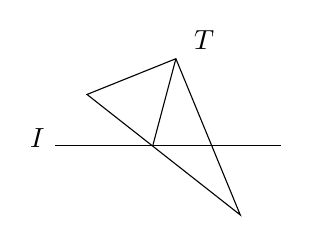
\begin{tikzpicture}[x=0.75pt,y=0.75pt,yscale=-1,xscale=1]
    %uncomment if require: \path (0,300); %set diagram left start at 0, and has height of 300
    %Straight Lines [id:da13049536652521132] 
    \draw    (111,120) -- (220,120) ;
    %Shape: Triangle [id:dp8829480866210793] 
    \draw   (169.14,78.09) -- (200.16,153.35) -- (126.32,95.31) -- cycle ;
    %Straight Lines [id:da19237153262125406] 
    \draw    (169.14,78.09) -- (158,120) ;
    % Text Node
    \draw (177,63.4) node [anchor=north west][inner sep=0.75pt]    {$T$};
    % Text Node
    \draw (98,110.4) node [anchor=north west][inner sep=0.75pt]    {$I$};
    \end{tikzpicture}
  \end{center}

we see that every triangle \(T\) which \(T \cap I \neq \varnothing\) can
be decomposed as the three smaller triangles which is covered by the
previous cases. We conclude that \(f\) is holomorphic in \(D\) by
Morera's theorem. \qed

\begin{theorem}[Schwarz Reflection Principle]
  Suppose that \(f\) is a holomorphic function in \(\Omega^+\) that extends 
  continuously to \(I\) such that \(f\) is real-valued on \(I\). Then, there exists 
  a function \(F\) holomorphic on \(\Omega\) such that \(F \mid_{\Omega^+} = f\).
\end{theorem}
\proof

Define \(F\) on \(\Omega^-\) by \(F(z) = \overline{f(\bar z)}\) for all
\(z \in \Omega^-\). Then to show that \(F\) is holomorphic in
\(\Omega^-\), we note that for all \(z, z_0 \in \Omega^-\), the
\(\bar z, \bar z_0 \in \Omega^+\), and hence, by Taylor expansion, we
have \[f(\bar z) = \sum_{n = 0}^\infty a_n (\bar z - \bar z_0)^n.\]
Thus,
\[F(z) = \overline{f(\bar z)} = \sum_{n = 0}^\infty \bar a_n(z - z_0)^n,\]
so \(F\) is holomorphic on \(\Omega^-\). With that, the result follows
by the symmetry principle. \qed

\hypertarget{complex-logarithm}{%
\subsection{Complex Logarithm}\label{complex-logarithm}}

We return to consider the logarithm as a single-valued function. As we
have seen, to define the complex logarithm, we had to restrict the set
which it is defined. Indeed, the definition we have seen thus far -- the
principle logarithm, restricted the domain to
\(\mathbb{C} \setminus (-\infty, 0]\). This is choice of restriction,
however, is rather arbitrary, and as we shall see now, the principle
logarithm is simply one of many choices of a \emph{branch} of the
logarithm.

\begin{theorem}
  Suppose \(\Omega\) is simply connected with \(1 \in \Omega\) and \(0 \not\in \Omega\). 
  Then, in \(\Omega\) there is a branch of the logarithm \(F(z) = \log_\Omega(z)\) 
  so that,
  \begin{itemize}
    \item \(F\) is holomorphic in \(\Omega\);
    \item \(e^{F(z)} = z\) for all \(z \in \Omega\);
    \item \(F(r) = \log r\) whenever \(r \in \mathbb{R}\) and sufficiently close 
      to \(1\).
  \end{itemize}
\end{theorem}

In other words, each branch \(\log_\Omega\) is an extension of the
standard logarithm defined for positive numbers.

\proof

We construct \(F\) as a primitive of the function
\(z \mapsto \frac{1}{z}\). Since \(0 \not\in \Omega\), the function
\(f(z) = 1 / z\) is holomorphic in \(\Omega\) and so, we may define
\[\log_\Omega(z) = F(z) = \int_\gamma f(z) \dd z,\] where \(\gamma\) is
any curve connecting \(1\) to \(z\). Since \(\Omega\) is simply
connected, this definition does not depend on the path chosen and thus,
this definition is well-defined. Now, \(F\) is holomorphic on \(\Omega\)
as it is the integral of a holomorphic function, and so, part 1 is
established.

For part 2, by rearranging, we see that it suffices to show
\(ze^{-F(z)} = 1\) for all \(z \in \Omega\). Consider,
\[\dv{z}(ze^{-F(z)}) = e^{-F(z)} - z F'(z)e^{-F(z)} = 
    (1 - z 1 / z) e^{-F(z)} = 0,\] and so \(ze^{-F(z)}\) is a constant.
Thus, as \(F(1) = 0\), we have \(ze^{-F(z)}\mid_{z = 1} = 1\), and so
\(ze^{-F(z)} = 1\) for all \(z\). \qed

\newpage

\hypertarget{meromorphic-functions}{%
\section{Meromorphic Functions}\label{meromorphic-functions}}

A meromorphic function on some domain \(\Omega\) is a holomorphic
function except at some isolated points in \(\Omega\). Meromorphic
functions are useful in that they are nicely behaved as, it turns out,
they can be written as a ratio between two holomorphic functions.

\hypertarget{laurent-series}{%
\subsection{Laurent Series}\label{laurent-series}}

Let us first consider an important expansion which shall aid us
throughout this chapter.

\begin{definition}[Laurent Series]
  A series 
  \[f(z) := \sum_{-\infty}^\infty a_n(z - z_0)^n\]
  is called a Laurent series for \(f\) at \(z_0\) whenever the series converges.
\end{definition}

\begin{theorem}[Laurent Expansion Theorem]
  Let \(f\) be holomorphic in the annulus \(D := \{z \mid r < |z - z_0| < R\}\) 
  for some \(z_0 \in \mathbb{C}\), \(r, R \in \mathbb{R}^+\). Then, \(f\) 
  can be expressed as 
  \[f(z) = \sum_{-\infty}^\infty a_n(z - z_0)^n,\]
  where
  \[a_n := \frac{1}{2\pi i} \ointctrclockwise_\gamma 
    \frac{f(\eta)}{(\eta - z_0)^{n + 1}} \dd \eta,\]
  and \(\gamma\) is any simple, closed, piecewise-smooth curve in \(D\) that 
  contains \(z_0\) in its interior.
\end{theorem}

We note that we consider a annulus rather a disk since as \(z \to z_0\),
the negative terms diverges to \(+\infty\). This allow us to consider
the Laurent expansion despite the presence of singularities since we can
simply centre the expansion such that the singularity is contained in
\(\{z \mid |z - z_0| < r\}\).

\proof

Wlog. assume \(z_0 = 0\) and define
\[\gamma_1 := \{z \mid |z| < R' < R\} \text{ and } 
    \gamma_2 := \{z \mid |z| > r' > r\}\] such that
\(z \in D' := \{ z \mid r' < |z| < R\}\). Then,
\[f(z) = \frac{1}{2\pi i} \ointctrclockwise_{\gamma_1} \frac{f(\eta)}{\eta - z} \dd \eta
    - \ointctrclockwise_{\gamma_2} \frac{f(\eta)}{\eta - z} \dd \eta := I_1 - I_2.\]
(This is the case since we may appropriate cuts between \(\gamma_1\) and
\(\gamma_2\)) Furthermore, if \(\eta \in \gamma_1\), then
\(|\eta| > |z|\) and so \(|z / \eta| < 1\), hence,
\[I_1 = \frac{1}{2\pi i}\ointctrclockwise_{\gamma_1} \frac{f(\eta)}{\eta - z} \dd \eta = 
    \frac{1}{2\pi i}\ointctrclockwise_{\gamma_1} \frac{f(\eta)}{\eta(1 - z / \eta)} \dd \eta 
    = \frac{1}{2\pi i}\sum_{n = 0}^\infty \ointctrclockwise_{\gamma_1} 
    \frac{f(\eta)}{\eta^{n + 1}} \dd \eta z^n \] where the last equality
is due to the geometric series.

On the other hand, for all \(\eta \in \gamma_2\) , \(|\eta| < |z|\) and
so
\[- I_2 = -\frac{1}{2\pi i}\ointctrclockwise_{\gamma_2} \frac{f(\eta)}{\eta - z} \dd \eta 
    = \frac{1}{2\pi i}\ointctrclockwise_{\gamma_2} \frac{f(\eta)}{z(1 - \eta / z)} \dd \eta
    = \frac{1}{2\pi i} \sum_{n = 0}^\infty \frac{1}{z^{n}} 
      \ointctrclockwise_{\gamma_2} f(\eta)  \eta^n \dd \eta.\] Thus, by
replacing parameters with \(- k := n + 1\), we have
\[- I_2 = \frac{1}{2\pi i} \sum_{k = - \infty}^{-1} 
    \ointctrclockwise_{\gamma_2} \frac{f(\eta)}{\eta^{k + 1}} \dd \eta z^k.\]
With that, putting these two integrals we have
\[f(z) = \sum_{-\infty}^\infty a_n z^n,\] with
\[a_n = \frac{1}{2\pi i} \ointctrclockwise_{\gamma_1} \frac{f(\eta)}{\eta^{n + 1}} \dd \eta,\]
for non-negative \(n\) and
\[a_n = \frac{1}{2\pi i} \ointctrclockwise_{\gamma_2} \frac{f(\eta)}{\eta^{n + 1}} \dd \eta,\]
for negative \(n\). Hence, the result follows by the deformation
theorem. \qed

\hypertarget{poles-and-zeros}{%
\subsection{Poles and Zeros}\label{poles-and-zeros}}

\begin{definition}[Zeros]
  We say a holomorphic function \(f : \Omega \to \mathbb{C}\) 
  has a zero of order \(m\) at \(z_0 \in \mathbb{C}\) is 
  \[f^{(k)}(z_0) = 0,\]
  for all \(k = 0, 1, \cdots, m - 1\), and \(f^{(m)}(z_0) \neq 0\).
\end{definition}

\begin{prop}
  A holomorphic function \(f\) has a zero of order \(m\) at \(z_0\) if and only 
  if it can be written in the form 
  \[f(z) = (z - z_0)^mg(z),\]
  for some \(g\) holomorphic at \(z_0\) and \(g(z_0) \neq 0\).
\end{prop}
\proof

We see that the reverse direction is true straight away, so let us
consider the forward direction. Suppose \(f\) has a zero of order \(m\)
at \(z_0\), then, since \(f\) is holomorphic, we may write \(f\) as a
Taylor expansion centred at \(z_0\). Indeed, by the definition of zeros,
we have the first \(m\) Taylor expansion terms vanishing while the
remaining terms all contain \((z - z_0)^m\). By factoring this outside
the sum, we have the required decomposition. \qed

While this proposition seems to be rather obvious, it has some striking
consequences.

\begin{corollary}
  The zeros of a non-constant holomorphic function are isolated, i.e. every 
  zero has a neighbourhood inside of which it is the only zero.
\end{corollary}
\proof

If \(z_0\) is a zero of order \(m\) of \(f\), then
\(f(z) = (z - z_0)^m g(z)\) where \(g\) is holomorphic at \(z_0\) and
\(g(z_0) \neq 0\). Then, \(g\) is continuous at \(z_0\) and therefore,
there exists a neighbourhood around \(z_0\) in which \(g(z) \neq 0\).
Thus, on this neighbourhood \(f(z) = (z - z_0)^m g(z) \neq 0\) except at
\(z_0\). \qed

\begin{definition}[Singularity]
  A point \(z_0\) is called a singularity of a complex function \(f\) if 
  \(f\) is not holomorphic at \(z_0\) but for every neighbourhood of \(z_0\) -- \(U\), 
  there exists some \(z \in U\) such that \(f\) is holomorphic at \(z\).
\end{definition}

\begin{definition}[Isolated]
  A singularity \(z_0\) of \(f\) is said to be isolated if there exists a neighbourhood 
  of \(z_0\) on which \(z_0\) is the only singularity of \(f\).
\end{definition}

\begin{definition}
  Let \(z_0\) be an isolated singularity of the holomorphic function \(f\) on some 
  domain. Then, if
  \[f(z) = \sum_{-\infty}^\infty a_n (z - z_0)^n\]
  is the Laurent expansion of \(f\) which is valid in some annulus \(0 < |z - z_0| < R\), 
  \begin{itemize}
    \item if \(a_n = 0\) for all \(n < 0\), then \(z_0\) is called a removable singularity;
    \item if \(a_n = 0\) for all \(n < -m\) where \(m \in \mathbb{Z}^+\) is fixed with 
      \(a_{-m} \neq 0\), then \(z_0\) is called a pole of order \(m\);
    \item if \(a_n \neq 0\) for infinitely many \(n \in \mathbb{Z}^-\), \(z_0\) is 
      called an essential singularity.
  \end{itemize}
\end{definition}

\begin{prop}
  A function \(f\) has a pole of order \(m\) at \(z_0\) if and only if it can be 
  written in the form 
  \[f(z) = \frac{g(z)}{(z - z_0)^m}\]
  where \(g\) is holomorphic at \(z_0\) and \(g(z_0) \neq 0\).
\end{prop}
\proof

If \(g\) is holomorphic at \(z_0\) and \(g(z_0) \neq 0\), then for some
\(R > 0\), \[g(z) = a_0 + a_1(z_1 - z_0) + \cdots,\] for all
\(z \in B_R(z_0)\) by Taylor expansion where \(a_0 = g(z_0) \neq 0\).
Then
\[f(z) = \frac{a_0}{(z - z_0)^m} + \frac{a_1}{(z - z_0)^{m - 1}} + \cdots,\]
for all \(z \in B_R(z_0) \setminus \{z_0\}\) and so \(z_0\) is a pole of
order \(m\).

Conversely, if \(f\) has a pole of order \(m\) at \(z_0\), then the
Laurent expansion of \(f\) is
\[f(z) = \frac{a_{- m}}{(z - z_0)^m} + \frac{a_{- m + 1}}{(z - z_0)^{m - 1}} + \cdots
    = \frac{1}{(z - z_0)^m}(a_{- m} + a_{- m + 1}(z - z_0) + \cdots),\]
which is a power series. Thus by defining
\[g(z) = a_{- m} + a_{- m + 1}(z - z_0) + \cdots,\] we have the required
function. \qed

\hypertarget{residue-theory}{%
\subsection{Residue Theory}\label{residue-theory}}

\begin{definition}[Residue]
  Let \(f\) be some complex function with the Laurent expansion at \(z_0\) 
  \[f(z) = \sum_{- \infty}^\infty a_n(z - z_0)^n,\]
  for \(z \in B_R(z_0) \setminus \{z_0\}\). Then, the residue of \(f\) at \(z_0\) 
  is 
  \[\text{Res}[f, z_0] = a_{-1}.\]
\end{definition}

\begin{prop}
  Let \(\gamma \subseteq \{z \mid 0 < |z - z_0| < R\}\) be a simple, closed, 
  piecewise-smooth curve such that \(z_0 \in \gamma^\circ\). Then 
  \[\text{Res}[f, z_0] = \frac{1}{2\pi i} \ointctrclockwise_\gamma f(z) \dd z.\] 
\end{prop}
\proof

Let \(0 < r < R\). Then, by the deformation theorem, we obtain
\[\begin{split}
    \frac{1}{2\pi i} \ointctrclockwise_\gamma f(z) \dd z 
    & = \frac{1}{2\pi i} \ointctrclockwise_{|z - z_0| = r} f(z) \dd z
      = \frac{1}{2\pi i} \ointctrclockwise_{|z - z_0| = r} 
        \sum_{- \infty}^\infty a_n(z - z_0)^n \dd z \\
    & = \frac{1}{2\pi i} \sum_{- \infty}^\infty 
        \int_0^{2 \pi} a_n r^n e^{i n \theta} i r e^{i \theta} \dd \theta
      = a_{-1},
  \end{split}\] where we parametrised \(z = re^{i \theta} + z_0\). \qed

\begin{prop}
  Let \(f\) be a holomorphic function inside and on a simple, closed piecewise-smooth 
  curve \(\gamma\) except at the singularities \(z_1, \cdots z_n\) in its interior. 
  Then 
  \[\ointctrclockwise_\gamma f(z) \dd z = 2\pi i \sum_{j = 1}^n \text{Res}[f, z_j].\]
\end{prop}
\proof

By the deformation theorem, the integral equals to the sum of curves
surrounded each of the singularities. Thus,
\[\ointctrclockwise_\gamma f(z) \dd z = \sum_{j = 1}^n \ointctrclockwise_{\gamma_j} f(z) \dd z,\]
for appropriate \(\gamma_j\). Hence, the result follows by the previous
proposition. \qed

This result allows us to evaluate complicated integrals. As an example,
consider the following integral,
\[\ointctrclockwise_{|z| = 1} e^{1 / z} \dd z.\] Clearly,
\[e^{1 / z} = 1 + \frac{1}{z} + \frac{1}{2!z^2} + \frac{1}{3!z^3} + \cdots,\]
and so, \(\text{Res}[e^{1 / z}, 0] = 1\) and hence,
\(2\pi i = \ointctrclockwise_{|z| = 1} e^{1 / z} \dd z\).

While this result is powerful, it is not always easy to compute the
Laurent coefficients explicitly. In this case, we may employ the
following method. Suppose \(f\) has a pole of order \(m\) at \(z_0\) and
let \(g(z) = (z - z_0)^m f(z)\). Then if \(m = 1\), we have
\[g(z) = a_{-1} + a_0(z - z_0) + \cdots,\] and so,
\[\text{Res}[f, z_0] = a_{- 1} = \lim_{z \to z_0} g(z) = \lim_{z \to z_0} (z - z_0)f(z).\]
Similarly, if \(m > 1\), we may simple derivate \(g\), \(m - 1\)-times
resulting in \(a_{- 1}\) being the first coefficient, allowing us to
apply the same argument, i.e.
\[\text{Res}[f, z_0] = \lim_{z \to z_0} \frac{1}{(m - 1)!} \dv[m - 1]{z}((z - z_0)^m f(z)).\]

\begin{theorem}[Principle of the Argument]
  Let \(f\) be holomorphic in an open set \(\Omega\) for a finite number of poles 
  and let \(\gamma\) be simple, closed, piecewise-smooth curve in \(\Omega\) 
  that does not pass through any poles or zeros of \(f\). Then 
  \[\ointctrclockwise_\gamma \frac{f'(z)}{f(z)} \dd z = 2 \pi i (N - P),\]
  where \(N\) and \(P\) are the sums of the orders of the zeros and poles of 
  \(f\) inside \(\gamma\) respectively.
\end{theorem}

The name of this theorem follows from the fact that
\[\frac{f'(z)}{f(z)} = \dv{z} \log(f(z)),\] and so,
\[\ointctrclockwise_\gamma \frac{f'(z)}{f(z)} \dd z = 
  \ointctrclockwise_\gamma \dv{z} \log(f(z)) \dd z = i\Delta \arg f(z).\]

\proof

If \(z_1\) is a zero of order \(n\), then \(f(z) = (z - z_1)^n g(z)\)
for some \(g\) holomorphic at \(z_1\) and \(g(z_1) \neq 0\).
Consequently, \[f'(z) = n(z - z_1)^{n - 1}g(z) + (z - z_1)^n g(z)\] and
\[\frac{f'(z)}{f(z)} = \frac{n}{z - z_1} + \frac{g'(z)}{g(z)}.\] Since
\(g(z_1) \neq 0\), there exists some neighbourhood \(B_r(0)\), such that
on which \(g \neq 0\) and hence, \(g'(z) / g(z)\) is holomorphic on
\(\{z \mid |z - z_1| < r\}\) and we have
\[\ointctrclockwise_{|z -z_1| < r}\frac{f'(z)}{f(z)} \dd z 
    = \ointctrclockwise_{|z -z_1| < r}\frac{n}{z - z_1} \dd z + 
      \ointctrclockwise_{|z -z_1| < r}\frac{g'(z)}{g(z)} \dd z = 2\pi i n.\]
Now, if \(z_2\) is a pole of order \(p\), then
\(f(z) = g(z) / (z - z_2)^p\) for some \(g\) holomorphic at \(z_2\) and
\(g(z_2) \neq 0\). Consequently,
\[f'(z) = \frac{-pg(z)}{(z - z_2)^{p + 1}} + \frac{g'(z)}{(z - z_2)^p},\]
and \[\frac{f'(z)}{f(z)} = \frac{-p}{z - z_2} + \frac{g'(z)}{g(z)}.\] By
the same argument, \(g' / g\) is holomorphic in a neighbourhood of
\(z_2\), and thus, again,
\[\ointctrclockwise_{|z -z_2| < r}\frac{f'(z)}{f(z)} \dd z 
    = \ointctrclockwise_{|z -z_2| < r}\frac{-p}{z - z_2} \dd z + 
      \ointctrclockwise_{|z -z_2| < r}\frac{g'(z)}{g(z)} \dd z = - 2\pi i p.\]
Thus, by the deformation theorem, the result follows. \qed

\begin{theorem}[Rouche's Theorem]
  Let \(f, g\) be holomorphic in an open set \(\Omega\) and let \(\gamma \subseteq \Omega\) 
  be a simple, closed, piecewise-smooth curve. If \(|g(z)| < |f(z)|\) for all 
  \(z \in \gamma\), then the sums of the orders of the zeros of \(f + g\) and 
  \(f\) inside \(\gamma\) are the same.
\end{theorem}
\proof

Consider the homotopy \(f_t(z) = f(z) + tg(z)\) for \(t \in [0, 1]\).
Suppose we let \(n(t)\) be the number of zeros of \(f_t\) inside
\(\gamma\) counted with multiplicities. Then inequality \(|f| > |g|\)
implies that, \(f_t\) has no zeros on \(\gamma\) and hence,
\[F_t(z) := \frac{f_t'(z)}{f_t(z)}\] has no poles on \(\gamma\).
Therefore, the argument principle implies
\[n(t) = \frac{1}{2\pi i}\ointctrclockwise_\gamma F_t(z) \dd z = 
    \ointctrclockwise_\gamma \frac{f_t'(z)}{f_t(z)} \dd z.\] Thus, since
\(n(t) \in \mathbb{Z}\), it suffices to show that \(n\) is continuous.
Indeed, since \(|f| > |g|\), we obtain that there exists some
\(\delta > 0\) such that \(|f_t| = |f + tg| \ge |f| - t|g| > \delta\)
for all \(t \in [0, 1]\). So, for any \(t_1, t_2 \in [0, 1]\), we have
\[\begin{split}
    |n(t_2) - n(t_1)| 
      & = \left| \frac{1}{2\pi i} \ointctrclockwise_\gamma \left(
            \frac{f'(z) + t_2 g'(z)}{f(z) + t_2 g(z)} - 
            \frac{f'(z) + t_1 g'(z)}{f(z) + t_1 g(z)}
          \right) \right|\\
      & \le \frac{1}{2\pi} \max_{z \in \gamma} \left| 
        \frac{(t_2 - t_1)(f(z)g'(z) - f'(z)g(z))}{(f(z) + t_2 g(z))(f(z) + t_1 g(z))}
        \right| \cdot \text{length } \gamma\\
      & \le \frac{C}{\delta^2}|t_2 - t_1|
  \end{split},\] where
\(C = \max_{z \in \gamma} f(z)g'(z) - f'(z)g(z)\). Thus, \(n\) is
continuous (in fact Lipschitz continuous) and the result follows by the
intermediate value theorem. \qed

\begin{definition}[Open Mapping]
  A mapping is said to be open if it maps open sets to open sets.
\end{definition}

\begin{theorem}[Open Mapping Theorem]
  If \(f\) is holomorphic and non-constant in an open set \(\Omega \subseteq \mathbb{C}\), 
  then \(f\) open.
\end{theorem}
\proof

Since a set is open if and only if it is locally open, we shall show
that for all \(w_0 \in \text{Im}f\), there exists a neighbourhood of
\(w_0\) also contained in \(\text{Im}f\).

Let \(w_0\) belong to the image of \(f\) such that \(f(z_0) = w_0\) and
suppose \(w\) is some number near \(w_0\). Defining \(g(z) := f(z) - w\)
we can write \[g(z) = (f(z) - w_0) + (w_0 - w) = F(z) + G(z).\] Choosing
\(\delta > 0\) such that \(\{z \mid | z - z_0 | \le \delta\}\) is
contained in \(\Omega\) and \(f(z) \neq w_0\) for
\(|z - z_0| = \delta\). Then, by selecting \(\epsilon > 0\) such that
\(|f(z) - w_0| \ge \epsilon\) on the circle \(|z - z_0| = \delta\), for
all \(|w - w_0| < \epsilon\), we have \(|F(z)| > |G(z)|\), and hence, by
Rouche's theorem, we conclude that \(g = F + G\) has only one zero
inside \(C_\delta\) since \(F\) has only one. Thus, there exists
uniquely \(z \in \Omega\) such that \(g(z) = f(z) - w = 0\), and so
\(w \in f(\Omega)\). \qed

\begin{theorem}[Maximum Modulus Principle]
  If \(f\) is a non-constant holomorphic function on an open set \(\Omega \subseteq \mathbb{C}\), 
  then \(|f|\) cannot attain a maximum in \(\Omega\).
\end{theorem}
\proof

Suppose \(f\) attained a maximum at \(z_0 \subseteq \Omega\). Since
\(f\) is holomorphic and non-constant, it is an open mapping, and thus,
if \(z_0 \in D \subseteq \Omega\) is open, \(f(D)\) is an open set
containing \(f(z_0)\). But then, there exists \(z \in D\) such that
\(|f(z)| > |f(z_0)|\), contradicting the maximality of \(f(z_0)\). \qed

\begin{corollary}
  Suppose \(f : \bar \Omega \to \mathbb{C}\) is continuous on \(\bar \Omega\) 
  and holomorphic on \(\Omega\) where \(\Omega \subseteq \mathbb{C}\) is open 
  and \(\bar \Omega\) is compact (equivalently, it is bounded). 
  Then, 
  \[\sup_{z \in \Omega}|f(z)| \le \sup_{z \in \bar \Omega \setminus \Omega} |f(z)|.\]
\end{corollary}

\newpage

\hypertarget{more-on-complex-valued-functions}{%
\section{More on Complex Valued
Functions}\label{more-on-complex-valued-functions}}

\hypertarget{harmonic-functions}{%
\subsection{Harmonic Functions}\label{harmonic-functions}}

\begin{definition}[Harmonic Function]
  Let \(\phi = \phi(x, y)\), \(x, y \in \mathbb{R}^2\) be a real function of two 
  variables. It is said to be harmonic in an open set \(\Omega \subseteq \mathbb{R}^n\) 
  if 
  \[\Delta \phi(x, y) := \pdv[2]{\phi}{x} + \pdv[2]{\phi}{y} = 
    \phi''_{xx} + \phi''_{yy} = 0.\]
  We usually refer \(\Delta\) as the Laplace operator.
\end{definition}

\begin{prop}
  Let \(f(x) = u(x, y) + iv(x, y)\) be holomorphic in an open set \(\Omega\). 
  Then \(u, v\) are harmonic function in \(\Omega\).
\end{prop}
\proof

Since \(f = u + iv\) is holomorphic it is infinitely differentiable. In
particular, the functions \(u, v\) have continuous second derivatives
that allows us to change the order of the second derivatives. Thus, by
the Cauchy-Riemann equations to obtain,
\[u''_{xx} = (u'_x)'_x = (v'_y)'_x = (v'_x)'_y = (-u'_y)'_y = -u''_{yy}.\]
Therefore, \[u''_{xx} + u''_{yy} = 0,\] and hence \(\Delta u = 0\) and
so, its harmonic. Similar argument shows that \(v\) is also harmonic.
\qed

\begin{theorem}[Harmonic Conjugate]
  Let \(u\) be harmonic in an open disc \(D \subseteq \mathbb{C}\). Then, there 
  exists some harmonic function \(v\), such that \(f := u + iv\) is holomorphic. 
  In this case, \(v\) is called a harmonic conjugate of \(u\).
\end{theorem}
\proof

Fix \(R > 0\) such that \(D = D_R\) and let \((x, y) \in D_R\),
\(\gamma = \gamma_1 \cup \gamma_2\) where
\[\gamma_1 := \{(t, s) \mid t \in (0, x), s = 0\},\]
\[\gamma_2 := \{(t, s) \mid t = x, s = (0, y)\}.\] Then, we construct
\(v\) such that
\[v(x, y) = \int_\gamma \left( - \pdv{u}{y} \dd t + \pdv{u}{x} \dd s\right).\]
Using \(u''_{xx} = -u''_{y}\), we obtain
\[v'_x(x, y) = - u'_y(x, 0) + \int_0^y \pdv[2]{u(x, s)}{x} \dd s 
    = - u'_y(x, 0) + \int_0^y \pdv[2]{u(x, s)}{s} \dd s.\] So, by FTC,
we have the above equals \(-u'_y(x, y)\). Now, differentiating with
respect to \(x\), we find
\[v'(x, y) = \pdv{y}\left(\int_\gamma \left( - \pdv{u}{y} \dd t + \pdv{u}{x} \dd s\right)\right) 
    = u_x'(x, y).\] Hence, by the Cauchy-Riemann equations are satisfied
and \(f\) is holomorphic. \qed

\begin{prop}
  Let \(f = u + iv\) be holomorphic on an open connected set \(\Omega \subseteq \mathbb{C}\). 
  Consider the two curves
  \[u(x, y) = C \text{ and } v(x, y) = K,\]
  where \(C, K\) are constants. Assuming the curves intercept at \((x_0, y_0)\) 
  and \(f'(z_0) \neq 0\) at \(z_0 = x_0 + iy_0\). Then, the curves are orthogonal 
  with respect to one another, i.e. \(\nabla u \cdot \nabla v = 0\).
\end{prop}
\proof

Clearly, \(u, v\) satisfies the Cauchy-Riemann equations, and so
\[\nabla u \cdot \nabla v = u'_x v'_x + u'_y v'_y = v'_yv'_x - v'_y v'_x = 0.\]
\qed

\hypertarget{conformal-mappings}{%
\subsection{Conformal Mappings}\label{conformal-mappings}}

Let us consider a smooth curve \(\gamma \subseteq \mathbb{C}\)
parametrised by \(z(t) = x(t) + iy(t)\) for \(t \in [a, b]\). For each
\(t_0 \in [a, b]\), we define the direction vector
\[L_{t_0} = \{(z(t_0) + tz'(t_0)) \mid t \in \mathbb{R}\}.\] Consider
now two curves \(\gamma_1\) and \(\gamma_2\) parametrised by the
functions \(z_1, z_2\) intersecting at \(t = 0\), namely
\(z_1(0) = z_2(0)\). Then we define the angle between the two curves to
be the angle between the tangents, that is
\[\arg z_2'(0) - \arg z_1'(0).\] We have the following result.

\begin{theorem}[Angle Preservation Theorem]
  Let \(f\) be holomorphic on an open subset \(\Omega \subseteq \mathbb{C}\). 
  Suppose that two curves \(\gamma_1\), \(\gamma_2\) are lying in \(\Omega\) 
  parametrised by \(z_1, z_2\) respectively. Assuming \(z_0 = z_1(0) = z_2(0)\) 
  is their intersection point and \(z_1'(0), z_2'(0)\) and \(f'(z_0)\) are all 
  non-zero. Then, the angle between the curves \((z_1, z_2)\) and \((f(z_1), f(z_2))\) 
  at \(t = 0\) satisfy, 
  \[\arg z_2'(t) - \arg z_1'(t) \mid_{t = 0} = 
    \arg (f(z_2(t)))' - \arg (f(z_1(t)))' \mid_{t = 0} \mod 2\pi.\]
\end{theorem}

\proof

The proof of this is rather straight forward. Indeed, we have
\[\frac{(f(z_1(t)))'}{(f(z_2(t)))'} \mid_{t = 0} = 
    \frac{f'(z_1(0))z_1'(0)}{f'(z_2(0))z_2'(0)} = 
    \frac{f'(z_0)z_1'(0)}{f'(z_0)z_2'(0)} = \frac{z_1'(0)}{z_2'(0)}.\]
Thus, the result follows by writing \(z = re^{i \theta}\). \qed

We remark that the condition \(f'(z_0) \neq 0\) is essential. By
considering the holomorphic function \(z \mapsto z^2\) and let
\(z_0 = 0\). Then, clearly, \(f(z_0) = 0\) while any other complex
number with non-zero argument doubles their argument under the function.
Thus, in the case the angle is not preserved.

Furthermore, we see that this theorem implies that the orientation is
also preserved. In general, preservation of angle does not imply the
orientation is preserved. Ineed, if we consider \(z \mapsto \bar z\), we
have a (nonholomorphic) function which preserves angle but not
orientation.

\begin{definition}[Conformal Mapping]
  We say a complex function \(f\) is conformal in an open set \(\Omega \subseteq \mathbb{C}\) 
  if it is holomophic in \(\Omega\) and if \(f'(z) \neq 0\) for all \(z \in \Omega\).
\end{definition}

\begin{definition}[Local Injection]
  A holomorphic function \(f\) is a local injection on an open set \(\Omega \subseteq \mathbb{C}\) 
  if for any \(z_0 \in \Omega\), there exists some 
  \[D := \{z \mid |z - z_0| < r\} \subseteq \Omega,\]
  such that \(f\mid_D\) is injective.
\end{definition}

\begin{prop}
  Let \(f : \Omega \to \mathbb{C}\) be holomorphic and a local injection, then 
  \(f'(0) \neq 0\) for all \(z \in \Omega\). 
\end{prop}
\proof

Suppose there exists some \(z_0 \in \Omega\) such that \(f'(z_0) = 0\).
Then, for some sufficiently small \(r > 0\), there is
\(\overline{D_r(z_0)} \subseteq \Omega\) such that
\[f(z) - f(z_0) = a(z - z_0)^k + g(z),\] for some \(a \neq 0\),
\(k \ge 2\), \(g = O(|z - z_0|^{k + 1})\), for all \(z \in D_r\). For
sufficiently small \(w_r \neq 0\), let us write
\[f(z) - f(z_0) - w = F(z) + G(z),\] where \(F(z) = a(z - z_0)^k - w\)
and \(G(z) = g(z)\). If \(r > 0\) and \(|w|\) small enough, then we have
\(|G(z)| < |F(z)|\) for all \(z \in C_r(z_0)\), and so, by Rouche's
theorem implies that \(f(z) - f(z_0) - w\) has at least two zeros in
\(D_r(z_0)\).

Now since the zeros of the holomorphic function are isolated and
\(f'(z_0) = 0\), then for a sufficiently small \(r\), it follows
\(f'(0) \neq 0\) for \(z \neq z_0\). Therefore the roots of
\(f(z) - f(z_0) - w\) are distinct. But this violates the injective
assumption. Hence \(f'\neq 0\). \qed

\begin{prop}
  The inverse of a conformal mapping is holomorphic.
\end{prop}
\proof

Let \(g := f^{-1}\) denote the inverse of \(f\) on its range \(V\).
Suppose \(w_0 \in V\) and \(w\) is sufficiently close to \(w_0\).
Assuming \(w = f(z)\) and \(w_0 = f(z_0)\) with \(w \neq w_0\), we find
\[\frac{g(w) - g(w_0)}{w - w_0} = \frac{1}{\frac{w - w_0}{g(w) - g(w_0)}} = 
    \frac{1}{\frac{f(z) - f(z_0)}{z - z_0}}.\] Since \(f'(z_0) \neq 0\),
letting \(z \to z_0\) allows us to conclude \(g\) is holomorphic at
\(w_0\) and \(g'(w_0) = 1 / f'(g(w_0))\). \qed

\begin{definition}[Möbius Transformation]
  A Möbius transformation (also known as a bilinear transformation) is a map 
  \[f(z) = \frac{a z + b}{cz + d},\]
  for some \(a, b, c, d \in \mathbb{C}\) and \(ad - bc \neq 0\).
\end{definition}

The condition \(ad - bc = 0\) is necessary since if otherwise, the
transformation is a constant, and hence is no longer a conformal
mapping.

It is clear that a Möbius transformation is holomorphic except at the
simple pole \(z = - d / c\) and it has derivative
\[f'(z) = \frac{ad - bc}{(cz + d)^2}.\] Clearly, \(f' \neq 0\), we have
\(f\) is conformal throughout \(\mathbb{C} \setminus \{- d / c\}\).

\begin{prop}
  The inverse of a Möbius transformation is a Möbius transformation and the composition 
  of Möbius transformations is also a Möbius transformation.
\end{prop}
\proof

Easy check. \qed

The Möbius transformations can be classified.

\begin{definition}
  A Möbius transformation is of type 
  \begin{itemize}
    \item (M1) if it is in the form \(z \mapsto az\);
    \item (M2) if it is in the form \(z \mapsto z + b\);
    \item (M3) if it is in the form \(z \mapsto z^{-1}\).
  \end{itemize}
\end{definition}

\begin{prop}
  Every Möbius transformation is a composition of transformations of type 
  (M1), (M2), and (M3).
\end{prop}

\end{document}
